\documentclass[11pt,oneside,%draft%
]{memoir}

% Packages

\usepackage[USenglish]{babel}
\usepackage[utf8]{inputenc}
\usepackage[T1]{fontenc}
\usepackage{textcomp}
\usepackage[dvipsnames]{xcolor}
\usepackage{IEEEtrantools}
\usepackage{graphicx}
\usepackage[gen]{eurosym}
\usepackage{verbatim}
\usepackage{tocloft}
\usepackage{microtype}
\usepackage{amsmath}
\usepackage{amsfonts}
\usepackage{amssymb}
\usepackage{amsthm}
\usepackage{listings}
\usepackage{braket}
\usepackage[hyphens]{url}
\usepackage{makeidx}
\usepackage[colorlinks=true,urlcolor=blue,linkcolor=blue,linktocpage=true]{hyperref}

\definecolor{listinggray}{gray}{0.9}
\definecolor{lbcolor}{rgb}{0.9,0.9,0.9}

\lstdefinelanguage{propositio}
    {morekeywords={I, N},
    sensitive=true,
    breaklines=true,
    breakatwhitespace=true,
}

\lstdefinelanguage{joukko}
    {morekeywords={I,N,V,K},
    sensitive=true,
    breaklines=true,
    breakatwhitespace=true,
}

\lstset{
	%language=python,
	%backgroundcolor=\color{black},
    basicstyle=\small\ttfamily\color[HTML]{000000},
    %lineskip=1pt,
    showstringspaces=false,
    keywordstyle=\color[HTML]{000080},
    commentstyle=\color[HTML]{006699},
    stringstyle=\color[HTML]{CC6600},
    identifierstyle=\color[HTML]{830300},
    %frame=single,
    %frameround=tttt
	%tabsize=4,
	%rulecolor=,
        %upquote=true,
        %aboveskip={1.5\baselineskip},
        %columns=fixed,
        %showstringspaces=false,
        %extendedchars=true,
        %breaklines=true,
        %prebreak = \raisebox{0ex}[0ex][0ex]{\ensuremath{\hookleftarrow}},
        %frame=single,
        %showtabs=false,
        %showspaces=false,
        %identifierstyle=\ttfamily,
}




% Book layout

\setstocksize{8.6in}{6in}
\settrimmedsize{8.6in}{6in}{*}
\setlrmarginsandblock{0.8in}{0.8in}{*}
\setulmarginsandblock{0.8in}{*}{1}
\setlength{\headsep}{0.22in}
\setlength{\footskip}{0.4in}
\fixpdflayout
\checkandfixthelayout
\renewcommand{\cftdot}{}
\setlength\cftparskip{1pt}

% Page styels

\makepagestyle{thphp}
\makeoddhead{thphp}{}{\rightmark}{}
\makeevenhead{thphp}{}{\leftmark}{}
\makeoddfoot{thphp}{}{{\thepage}}{}
\makeevenfoot{thphp}{}{{\thepage}}{}

\makepagestyle{alku}
\makeoddhead{alku}{}{}{\leftmark}
\makeevenhead{alku}{\leftmark}{}{}
\makeoddfoot{alku}{}{}{{\thepage}}
\makeevenfoot{alku}{{\thepage}}{}{}

\pagestyle{thphp}

% Custom environments

\newenvironment{eqna}{\begin{IEEEeqnarray}{c}}{\end{IEEEeqnarray}\ignorespacesafterend}
\newenvironment{eqnb}{\begin{IEEEeqnarray}{rCl}}{\end{IEEEeqnarray}\ignorespacesafterend}
\newtheorem{teoreema}{Theorem}
\newtheorem{lemma}{Lemma}
\theoremstyle{definition}
\newtheorem{maaritelma}{Definition}



% Custom commands

\newcommand{\tip}{\vspace{0.2in}\noindent\textbf{TI}\quad}
%\newcommand[1]{\set}{\lbrace
\newcommand{\NN}{\mathbb{N}}
\newcommand{\RR}{\mathbb{R}}
\newcommand{\CC}{\mathbb{C}}
\newcommand{\ZZ}{\mathbb{Z}}
\newcommand{\KK}{\mathbb{K}}
\newcommand{\QQ}{\mathbb{Q}}
\newcommand{\dd}{\mathrm{d}}
\newcommand{\ee}{\mathrm{e}}
\newcommand{\ii}{\mathrm{i}}
\DeclareMathOperator{\Tr}{Tr}
\newcommand{\propositio}{\lstinline[language=propositio]}
\newcommand{\joukk}{\lstinline[language=joukko]}

\begin{document}

\frontmatter

\thispagestyle{empty}

\noindent{\HUGE\textbf{Reason}}

\vspace{0.3in}

\noindent Konsta Kurki

\vspace{0.3in}

\noindent In progress---updated on September 1, 2016

\vfill

\noindent\emph{This book is about fascinating things. I write about important things in my other free book \emph{Revolution}.\footnote{\url{http://www.revolution.fyi}} Please consider reading it before entertaining yourself with this book.}

\vfill
%\vspace{0.3in}

\noindent Copyright {\textcopyright} 2016 Konsta Kurki

\vspace{0.18in}

\noindent This book is licensed under a Creative Commons Attribution-ShareAlike 4.0 International License.\footnote{\url{https://creativecommons.org/licenses/by-sa/4.0/}} See the book webpage\footnote{\url{http://konstakurki.co/reason/}} for the source repository and the newest version and author's personal site\footnote{\url{http://konstakurki.co/}} for contact information.

\newpage

\mainmatter

\tableofcontents
%REMEMBER TO USE TAU INSTEAD OF 2PI

\chapter{Questions}

From the very childhood we all ask questions. We are curious and we search for answers. Here are some questions that fascinate me.

\begin{enumerate}
    \item Where do we come from?
    \item Is it possible to comb a hairy ball?
    \item Can we deduce every truth?
    \item Can we travel to the future?
    \item Can we build a universal computing machine?
    \item Can we send messages in obscure form?
    \item Why do people do mathematics?
    \item Can we build humane machines?
    \item Can we order the points of a line?
    \item Can we always choose?
    \item What separates future from the past?
    \item Is there present outside here?
    \item Are patents good?
    \item Why do heartless people exist?
    \item Can we describe physics in compact form?
    \item What is gravity?
    \item What is matter?
    \item What is heat?
    \item What is love?
    \item Will two straight parallel lines stay parallel?
    \item Is exact cloning possible?
    \item Is teleportation possible?
    \item Can we travel as fast as we want?
    \item What is the meaning of life?
\end{enumerate}

We came from the stars. That is poetic, yet true, yet vague statement. 

\begin{comment}

And here are some open ones.

\begin{enumerate}
    \item What happens if we squeeze stuff more and more?
    \item Is there a consistent axiom set for all mathematics? (?)
    \item Can we travel to the past?
    \item What was in the beginnign of the Big Bang and,
    if it's legitimate to ask, before it?
    \item What is our, life's and our Universe's faith?
    \item Is is possible to answer these questions without
    fucking one's brain up?
\end{enumerate}

\emph{We came from the stars.} That poetic verse? is how I answer the first one. But why would you believe me? Maybe you think I’m a good-willing guy, and you believe I wouldn’t lie to you. But even if that’s true, I may have mistaken and given you incorrect information accidentally.

Luckily, I can do better. I can <em>reason</em>. I can guide you so that you will understand, and you will end up thinking, ’we came from the stars’. Actually, you’ll end up with a much detailed picture, and you’ll end up there by your own thinking. There’s no need for you to believe me, no need for you to trust me. 

To be honest, I hope you do believe me in one thing: that you should read on. But if someone else has said that to you and you believe him or her, then you don’t need to believe me even about that. You don’t need to believe me at all, and that’s nice: it’s a damn heavy burden to take responsibility of truth. A person with a 1000-pound rock tied to the back only has theoretical freedom.

In this book I’ll build answers to questions in the list. Some will get a definite ’yes’ or ’no’ answer. Some will get more wordy, yet comprehensive answers. Some will be left open. I’ll discuss such questions so that you can get started, if you wish to find an answer.

More precisely, I mostly use common knowledge on which we all agree, like ’an apple likes to fall down to ground’. I use mathematics which makes common sense and which you can verify through Internet, and in some cases I quote empirical research supported by the strong consensus. If there’s a possibility of a flaw, I’ll point that out.

The questions may seem to be very different in their kinds. Some are mathematical, some consider natural science, and some are about humanity. According to the reader, some may be ridiculous, boring, impossible or philosophical. This book will show that these questions are, or with a little reformulation can be made, well-posed and answerable with the common sense we use for everyday purposes like deciding how to pack stuff in a backpack.

The road will be long and difficult. Populism isn’t of help here—we need to work through logic, computability theory, mathematics like topology, algebra, analysis and probability, physical theories like quantum mechanics, thermodynamics and relativity, and empirical data from cosmology, biology and psychology.


%Mä tässä mietin jo seuraavaa kirjaa. Se ei tule käsittelemään maailmanparannusta, vaan ymmärtämistä. Mä ajattelin että sen punainen lanka voisi olla muutaman kysymyksen joukko johon kirjan sivuilla vastataan. Tässä eräs luonnos tuosta joukosta:
%
%1.  Mistä me ihmiset tulemme?
%Primordial soup \& Big Bang.
%
%2.  Voiko karvaista palloa kammata?
    %Ei, jos haluaa siistin kampauksen: vähintään
    %yksi ryppypiste muodostuu (hairy ball theorem).
%
%3.  Onko teleportaatio mahdollista?
    %On jos käytössä on lomittunu EPR-tilapari
    %(quantum teleportation).
%
%4.  Miten menneisyys eroaa tulevaisuudesta?
    %Entropia kasvaa tulevaisuuteen ja pienenee
    %menneisyyteen päin (2. law of thermodynamics \&
    %the arrow of time).
%
%5.  Voimmeko rakentaa humaaneja koneita?
    %Komputationaaliset resurssit ja data ei
    %riitä siihen että kone voisi imeä ihmisyyttä
    %kovinkaan paljoa itseensä.
%
%6.  Onko täsmällinen kloonaaminen mahdollista?
    %Ei (no-cloning theorem, käsittääkseni
    %ratkaisee myös aaltofunktion
    %romahtamisongelman).
%
%7.  Voiko janan pisteet järjestää?
    %Ei luonnollisten lukujen avulla; valinta-
    %aksiooma implikoi well-ordering teoreeman
    %joka sanoo että on olemassa järjestys jossa
    %joka luvulla on seuraaja.
%
%8.  Voimmeko matkustaa tulevaisuuteen?
    %Kyllä, aivan kuinka kauas vain halutaan,
    %jos käytössä on tarpeeksi nopea
    %avaruusraketti tai musta aukko.
%
%9.  Voimmeko päätellä jokaisen totuuden?
    %Ei, 
%
%10. Mikä on elämän tarkoitus?
    %Termodynamiikan toista pääsääntöä vastaan
    %taisteleminen.
%
%Näihin kysymyksiin aukottomasti tai edes jokseenkin vakuuttavasti ei ole helppoa. Mahdollista se kuitenkin on.
%
\end{comment}

\part{Building math}

\chapter{Numbers}

We all use some math: numbers. To get into them, we start from sets. The set of living people, the set of grains of salt in a jar, the set of up and down, which we might denote by \(\lbrace\uparrow,\downarrow\rbrace\). % määritelmiä ja merkintöjä kuten unioni, leikkaus, functio yms.
%We all use numbers.

%\section{\(\NN\), \(\ZZ\), \(\QQ\), \(\RR\) and \(\CC\)}
\section{Counting things}

An elementary question about any set is, ``how many elements it has?'' The answer is called the cardinality of the set. For instance, the cardinality of \(\lbrace\uparrow,\downarrow\rbrace\), denoted by \(|\lbrace\uparrow,\downarrow\rbrace|\), is two. If two sets \(A\) and \(B\) have the same cardinality, we can put the elements of \(A\) in one-to-one correspondence with the elementes of \(B\), in other words, there's a bijective function \(f:A\rightarrow B\). %If \(\lbrace\uparrow,\downarrow\rbrace\) and \(B=\lbrace\leftarrow,\rightarrow\rbrace\),

This also works the other way around: if there's a bijection between \(A\) and \(B\), then \(|A|=|B|\). If there's a surjection from \(A\) to \(B\), then \(|A|\geq|B|\), and if there's an injection from \(A\) to \(B\), then \(|A|\leq|B|\). If there are both an injection and a surjection from \(A\) to \(B\), then \(|A|=|B|\), and there also is a bijection between \(A\) and \(B\).

A picture\footnote{\url{https://en.wikipedia.org/wiki/Bijection\%2C_injection_and_surjection}} makes these points clear, at least if \(A\) and \(B\) are finite. They also hold for infinite sets, but reasoning is more difficult. It for example takes some effort to show that if there's a surjection and an injection from \(A\) to \(B\), then there's also a bijection between them.\footnote{\url{https://en.wikipedia.org/wiki/Schr\%C3\%B6der\%E2\%80\%93Bernstein_theorem}}

The possible cardinalities of finite sets, \(0\), \(1\), \(2\), \(3\) and so on, are mathematical objects called natural numbers. They form another set called \(\NN\). It is an infinite set of which cardinality is denoted by \(\aleph_0\).

If we also count backwards from \(0\), we get
\begin{eqna}
    \ZZ=\lbrace\dotsc,-3,-2,-1,0,1,2,3,\dotsc\rbrace,
\end{eqna}
the set of integers. We end up with integers when we construct a set of results to every subtraction of natural numbers. There's a bijection between \(\ZZ\) and \(\NN\): by ordering the integers into a sequence
\begin{eqna}
    0,1,-1,2,-2,3,\dotsc
\end{eqna}
we can put them in one-to-one correspondence with \(\NN\). Therefore  \(|\ZZ|=\aleph_0\).

If we can count the elements of a set \(X\) by using \(\NN\), then \(X\) is said to be countable. To be precice, \(X\) is countable if there is a surjection \(f:\NN\rightarrow X\), that is, \(|X|\leq\aleph_0\). Finite sets and \(\aleph_0\) sets are countable.

Given any set \(X\), we can form a set of all its subsets. That set is called the power set of \(X\) and is denoted by \(2^X\). For example,
\begin{eqna}
    2^{\lbrace\uparrow,\downarrow\rbrace}=\lbrace\emptyset,\lbrace\uparrow\rbrace,\lbrace\downarrow\rbrace,\lbrace\uparrow,\downarrow\rbrace\rbrace,
\end{eqna}
in which \(\emptyset=\lbrace\,\rbrace\) denotes the empty set.

We have
\begin{eqna}
    |\lbrace\uparrow,\downarrow\rbrace|=2<4=|2^{\lbrace\uparrow,\downarrow\rbrace}|.
\end{eqna}
This seems plausible: there's much more possibilities in choosing elements from any set \(X\) than it has elements, so \(|X|<|2^X|\). Actually, if \(X\) is finite, then \(|2^X|=2^{|X|}\), since each element of \(X\) contributes a factor of two to the number of possible subsets.

We can also show this more carefully. Let \(X\) be any set, finite or infinite, and take any function \(f:X\rightarrow 2^X\). Then form a set
\begin{eqna}
    D=\lbrace x\in X: x\notin f(x)\rbrace.
\end{eqna}
The notation on the right means ``all real numbers \(x\) such that \(x\) is not in \(f(x)\).'' Is there a \(x\in X\) so that \(f(x)=D\)? If \(x\in f(x)\), then by the construction of \(D\) we have \(x\notin D\) and therefore \(f(x)\neq D\), and if \(x\notin f(x)\), then by the construction of \(D\) we have \(x\in D\), so \(f(x)\neq D\). In either case \(f(x)\neq D\), so \(f\) is not a surjection.

Since \(f\) was arbitrary, there's no surjection from \(X\) to \(2^X\), and so \(|X|<|2^X|\). We denote \(|2^X|\) by \(2^{|X|}\), which is in line with the corresponding result for finite sets.

This means that there are infinities of different sizes, so to speak. Actually, we have infinitely many of them:
\begin{eqna}
    \NN,\: 2^\NN,\: 2^{2^\NN},\:2^{2^{2^\NN}},\: \dotsc
\end{eqna}

Now take \(X\) to be the set of all sets. Such a set contains all its subset, so \(2^X\subset X\). This means that \(|2^X|\leq|X|\). We seem to have a contradiction here. The ``set of all sets'' is a problematic concept and we shall not use it.

Another too peculiar set is
\begin{eqna}
    R=\lbrace x:x\notin x\rbrace.
\end{eqna}
Does it hold that \(R\in R\)? If so, then by the definition of \(R\) we have \(R\notin R\)---and the other way around. This is a problem called Russel's paradox. The pradox can also be put in everyday language:
\begin{quote}
    In a village there's a man called Russell. He maintains GNU+Linux systems of some villagers. To be more specific, Russell maintains the GNU+Linux system of every villager who doesn't maintain their own system. An unsolved riddle puzzles the villagers: does Russell maintain his own GNU+Linux system?
\end{quote}
If Russel maintains his own system, then he maintains the system of a person who maintains his own system, sot that can't be true. On the other hand, if don't do that, then he does not maintain the system of every veillager not maintaining their own system.

The resolution of this parctical version is simple: no such Russell exists. In the same way, the set \(R\) does not exist. Russell, \(R\) and the set of all sets demonstrate that some caution is needed in defining sets.

Back to numbers. We can define natural numbers in terms of sets:
\begin{eqna}
    0=\emptyset,\quad 1=\lbrace0\rbrace,\quad2=\lbrace0,1\rbrace,\quad3=\lbrace0,1,2\rbrace
\end{eqna}
and so on. Every number is founded? on \(\emptyset\), for example
\begin{eqna}
    3=\lbrace\emptyset,\lbrace\emptyset\rbrace,\lbrace\lbrace\emptyset\rbrace\rbrace\rbrace.
\end{eqna}
For any natural number \(n\) it holds that \(n+1=n\cup\lbrace n\rbrace\). In this sense we can think of \(\NN\) as another number! In this context it is denoted by \(\omega\).  We can count even further:
\begin{eqna}
    \omega+1=\omega\cup\lbrace\omega\rbrace=\lbrace1,2,3,\dotsc,\lbrace1,2,3,\dotsc\rbrace\rbrace.
\end{eqna}
Numbers formed this way are called ordinals. \(\omega\) is the first infinite ordinal. At first it seems obvious that ordinals form a set \(O\). But \(O\) is also an ordinal number, just like \(\NN\), and therefore is also \(O+1=O\cup\lbrace O\rbrace\). On the other hand, \(O+1\in O\), but that seems weird; for example \(3\notin 2\). The set of all ordinals is flawed in the same way as the set of all sets.

This naive set theory doesn't work well for studying these issues. In more advanced treatments ordinals form so-called proper class, as do all sets?. Proper classes are ``too large'' to be sets.

If we place all integers equidistantly in a row which extends infinitely far both left and right, we get a sketch of the number line. The number line symbolizes size, distance, amount and other continuous quantities. \(\ZZ\) only forms a sparse part of the whole line. If we take all the points, we get \(\RR\), the set of real numbers, also called the continuum. Let's take a question from the list presented in the first chapter.
\begin{quote}
    Can we order the points of a line?
\end{quote}
More precicely, can we put all the real numbers in a row so that each \(x\in\RR\) always has a definite successor? The real number line clearly is not such a row---what would be the successor of \(0\) on the line? \(0.1\)? No, since there are real numbers between \(0\) and \(0.1\). To my personal intuition the task seems difficult. There's too many numbers in \(\RR\), I think.

On the other hand, if \(\RR\) is countable, we can order it by simply counting its elements.

Many points along the number line can be expressed as fractions, in the form \(x=\frac{m}{n}\) in which \(m,n\in\ZZ\). Such numebers are called rational numbers and their set is denoted by \(\QQ\). Between any two rational numbers \(q_1=\frac{m_1}{n_1}\) and \(q_2=\frac{m_2}{n_2}\), no matter how close to each other they are, there is another rational number
\begin{eqna}
    q_3=\frac{1}{2}q_1+\frac{1}{2}q_2=\frac{m_1n_2+m_2n_1}{2n_1n_2}.
\end{eqna}
Rational numbers are therefore very densely spaced on the number line. It seems that ordering \(\QQ\) is as difficult as ordering \(\RR\).

Consider the the Cartesian product \(\ZZ\times\ZZ\doteq\ZZ^2\), the set of ordered pairs \((m,n)\) in which \(m,n\in\ZZ\). We can form a function \(f:\ZZ^2\rightarrow\QQ\) which takes \((m,n)\mapsto\frac{m}{n}\), unless \(n=0\), in wich case we may define \((m,n)\mapsto 0\). Some pairs map to same rational numbers, for example \((1,2)\mapsto\frac{1}{2}\) and \((2,4)\mapsto\frac{2}{4}=\frac{1}{2}\), but for each \(q\in\QQ\) there is some pair that maps to it. In other words, \(f\) is a surjection and \(|\QQ|\leq|\ZZ^2|\). If we can count \(\ZZ^2\), we can also count \(\QQ\).

To count \(\ZZ^2\), draw a square grid in which the first \(\ZZ\) acts as the horizontal and the second as the vertical coordinate. Then start from the origin and spiral away to infinity. The resulting sequence,
\begin{eqna}
    (0,0),(1,0),(1,1),(0,1),(-1,1),(-1,0),\dotsc% piirrä kuva
\end{eqna}
defines a bijection \(f:\NN\rightarrow\ZZ^2\).

Here we have four infinite sets, \(\NN\subset\ZZ\subset\QQ\) and \(\ZZ^2\), each of them having cardinality \(\aleph_0\). If \(\RR\) is more or less like \(\QQ\), perhaps equal to it, then we can also count and order it. %Is there an infinite set X with |X| < aleph_0 ?

Let's investigate the issue. Take the interval
\begin{eqna}
    I=[0,1[\;\doteq\lbrace x\in\RR : 0\leq x<1\rbrace.
\end{eqna}
There's a surjection from \(I\) to \(\RR\) (take for example \(]0,1[\,\subset I\), stretch it to fill the whole \(\RR\) by a \(\tan(x)\)-like function and map \(0\) to \(0\)) and an injection (the trivial \(x\mapsto x\)), so \(|I|=|\RR|\). To find the cardinality of \(\RR\) it is enough to study \(I\).

Any \(x\in I\) is either smaller than \(\frac{1}{2}\) or greater or equal to \(\frac{1}{2}\), so it belongs to either \([0,\frac{1}{2}[\) or \([\frac{1}{2},1[\), that is, it belongs either to the forst or the socond half of \(I\). Say \(x\in[0,\frac{1}{2}[\). Then we can ask the same question again: is \(x\) in \([0,\frac{1}{4}[\) or \([\frac{1}{4},\frac{1}{2}[\)? This time \(x\) was found in the right interval. We continue and get an infinite sequense, ``left, right\ldots'', or \((\leftarrow,\rightarrow,\dotsc)\).

Therefore, for any \(x\in I\) we have an infinite sequence \(S_x\) of \(\leftarrow\)'s and \(\rightarrow\)'s. On the other hand, any such sequence determines an \(x\in I\)---if we turn any arrow around in the sequence, the corresponding number changes. Each sequence corresponds to exactly one \(x\in I\). We have constructed a bijection between \(I\) and the set of sequences \(S_x\).

Furthermore, a sequence \(S_x\) defines a subset of \(\NN\) if we take \(\rightarrow\) to mean ``does belong to the subset'' and \(\leftarrow\) to ``doesn't''. For example the sequence \((\rightarrow,\leftarrow,\rightarrow,\leftarrow,\leftarrow,\dotsc)\), with all the rest being \(\leftarrow\)'s, corresponds to the set \(\lbrace0,2\rbrace\). Therefore we've constructed a bijection between the sequences \(S_x\) and \(2^\NN\).

Putting these together, we have \(|\RR|=2^{|\NN|}\). \(\QQ\neq\RR\); \emph{\(\RR\) is uncountable.} Even though we could order \(\QQ\) by counting it using \(\NN\), we can't do the same to \(\RR\). Anyway, at least in principle there may be some other way to order \(\RR\).

Is there a set \(X\) such that \(\aleph_0<|X|<2^{\aleph_0}\)? So-called continuum hypothesis states that no such \(X\) exists. Is continuum hypothesis true is a sublte issue. Fortunately, it rarely matters. In most cases all that mattes is that is a set finite, countably infinite or uncountable.

%\begin{eqna}
    

%For any function \(f:\NN\mapsto\mathcal{S}\) we can form a table of the following form:
%\begin{eqna}
%\begin{array}{c|ccccc}
    %%%x_0 & \leftarrow  & \rightarrow & \leftarrow  & \leftarrow  & \cdots \\
    %x_1 & \leftarrow  & \leftarrow  & \leftarrow  & \rightarrow & \cdots \\
    %x_2 & \rightarrow & \rightarrow & \rightarrow & \rightarrow & \cdots \\
    %x_3 & \leftarrow  & \rightarrow & \leftarrow  & \leftarrow  & \cdots \\
    %\vdots & \vdots   & \vdots      & \vdots      & \vdots      & \ddots
%%\end{array}
%\end{eqna}
%Now, take the sequence that has appered on the diagonal and turn each of its arrows around. In this case we would get
%\begin{eqna}
    %(\rightarrow,\rightarrow,\leftarrow,\rightarrow,\dotsc).
%\end{eqna}
%Is this sequence somewhere in the table? No! If you try to fit it into the table, the arrow on the diagonal will always point into the wrong direction. Therefore, \(f\) is not a surjection. Since \(f\) was arbitrary, this means that there is no surjection from \(\NN\) to \(\mathcal{S}\) and so \(|\mathcal{S}|>\aleph_0\). The sets \(\mathcal{S}\), \(I\), \(\RR\) and \(2^\NN\) are uncountable and their cardinality is denoted by \(2^{\aleph_0}\), in line with the face that for a finite set \(X\) we have \(|2^X|=2^{|X|}\).
%
%We've seen that the power set of infinite \(\NN\) is strictly greater than \(\NN\) and that our speculation that every infinite set had cardinality \(\aleph_0\) was wrong. Instead, there are at least two infinities of different sizes: the countable \(\NN\) and the uncountable \(\RR\). We can't order real numbers by counting them with natural numbers.
%
%Actually, we can show that for any set \(X\) it holds that \(|X|<|2^X|\). Take any function \(f:X\rightarrow 2^X\). Then form a set
%\begin{eqna}
    %Y=\lbrace x\in X: x\notin f(x)\rbrace.
%\end{eqna}
%Is there a \(x\in X\) so that \(f(x)=Y\)? If \(x\in f(x)\), then by the construction of \(Y\) we have \(x\notin Y\) and therefore \(f(x)\neq Y\), and if \(x\notin f(x)\), then by the construction of \(Y\) we have \(x\in Y\), so \(f(x)\neq Y\). In either case \(f(x)\neq Y\), so \(f\) is not a surjection. Since \(f\) was arbitrary, there's no surjection from \(X\) to \(2^X\), and so \(|X|<|2^X|\).
%
%%\section{\texorpdfstring{\(\QQ\)}{Q} or something even more?}
%
%% shittii
%
%
%Let's collect the results. We have
%\begin{eqna}
    %|\NN|=|\ZZ|=|\ZZ^2|=|\QQ|=\aleph_0<|I|=|\RR|=|2^{\NN}|=2^{\aleph_0}.
%\end{eqna}






%Now assume that we have an ordered subset \((x_0,x_1,x_2\) of \(I\). We can put the corresponding sequences in a table:
%\begin{tabular}{c | c c c c}
    %\(x_0\) & \leftarrow & \rightarrow & \rightarrow & \cdots \\
    %\(x_0\) & \leftarrow & \rightarrow & \rightarrow & \cdots
%\end{tabular}
%\begin{eqna}
    %yeah
%\end{eqna}
%If we now take the sequence on the diagonal and turn each of its arrows around, we get another sequence and the corresponding number. In this example listing it would be \((\rightarrow,\rightarrow,\leftarrow,\dotsc)\). Is this number listed? No! It can't be anywhere in the listing, since the arrow that happens to be on the diagonal is turned around.

%So, given any listing of real numbers on the line \(I\), there's a number that isn't listed. In other words, we can't order \(I\) like we can order natural numbers and fractions---we can't count them. It's said that \(\NN\), \(\ZZ\) and fractions, or rational numbers, denoted by \(\QQ\), are countable, and \(I\) is uncountable. And, because \(I\subset\RR\), also \(\RR\) is uncountable. %we can identify the arrow lists to subsets of N and therefore see that R is of the same cardinality of 2^R. I should show that I is of the same cardinality as R, althoug it seems obvious. Furthermore, power set is always larger than the original and so the set of all sets seems problematic.

%Let's compare \(\QQ\) and \(\RR\). They're similar in the sense that they both are dense. This fact may trick intuition to assume that \(\QQ=\RR\). But sinse \(\RR\) is uncountable, it is larger than countable \(\QQ\). \(\RR\) has a larger cardinality than \(\QQ\), so our earlier notion that all infinite sets have cardinality \(\infty\) was flawed. The cardinaluty of \(\QQ\) is 

%\(\ZZ\) is also countable: it's easy to find a bijection to \(\NN\), it's just \((0,1,-1,2,-2,\dotsc)\). The cardinalities of two sets are same, if there is a bijection between them. The cardinality of all infinite countable sets is denoted by \(\aleph_0\). The cardinality of \(\RR\) is denoted by \(\mathfrak{c}\).

well-ordering here

%So the answer to the question if we can order the points of a line is:
%\begin{quote}
    %We cannot count points on a line by putting them in a corresponence with natural numbers \(0,1,2\) and so on. This is because \(\RR\) is an uncountable set. However, if we assume that we can always choose elements from sets, that is we embrace the Axiom of Choice, then we can prove that there exist an order in which every point has a definite successor.
%\end{quote}

\section{Rationals, reals or something more?}

The uncountability of \(\RR\) may seem peculiar. You might ask, ``wouldn't \(\QQ\) be enough for all practical purposes?'' One discomfortable property of any countable subsetset \(X=\lbrace x_i\in\RR : i\in\NN\rbrace\) of \(\RR\) like \(\QQ\) is that we can cover it using almost nothing. To do it, take a collection \(\lbrace I_i : i\in\NN\rbrace\) of intervals
\begin{eqna}
    I_0=\left[x_0,x_0+\tfrac{1}{2}c\right],\quad I_1=[x_1,x_1+\tfrac{1}{4}c],\,\dotsc
\end{eqna}
with \(c\in\RR\). The intervals clearly cover \(X\); in symbols,
\begin{eqna}
    X\subset\bigcup_{i\in\NN}I_i.
\end{eqna}
The length of the interval halves every time we go one step further in the sequence \(I_i\). The first interval has length \(\frac{1}{2}c\), the second \(\frac{1}{4}c\) and so on. If we juxtapose all these \(I_i\)'s in a row, we get a line that looks like
\begin{eqna}
    \setlength{\unitlength}{0.6666\textwidth}
    \begin{picture}(1,0.025)
        %\put(0,0){\vector(1,0){0.5}}
        %\put(0.5,0){\vector(1,0){0.25}}
        %\put(0.5,0){\vector(1,0){0.25}}
        \put(0,0.025){\line(1,0){1}}
        \put(0,0){\line(0,1){0.05}}
        \put(0.5,0){\line(0,1){0.05}}
        \put(0.75,0){\line(0,1){0.05}}
        \put(0.875,0){\line(0,1){0.05}}
        \put(0.9375,0){\line(0,1){0.05}}
        \put(0.96875,0){\line(0,1){0.05}}
        \put(0.984375,0){\line(0,1){0.05}}
        \put(0.9921875,0){\line(0,1){0.05}}
        \put(0.99609375,0){\line(0,1){0.05}}
        \put(0.998046875,0){\line(0,1){0.05}}
        \put(0.9990234375,0){\line(0,1){0.05}}
    \end{picture}.
\end{eqna}
Their sum is exaclty \(c\). The Greek philosopher Zeno of Elea was worried that if you are about to travel to a neighboring village, you muts first get halfway there. But to get halfway there, you must get quarter of the way there, and so on, \emph{ad infinitum}.

So, even though the number line is infinitely long and rational numbers are densely spaced on it, we can cover them with lines of which combined length is \(c\) which can be anything, for example \(\frac{1}{1000}\). This sounds paradoxal, but it should be kept in mind that had we used a finite collection of lines to cover \(\QQ\), then their combined length would have necessarily been \(\infty\).%any uncountable sum of positive terms is necessarily infinite?

It is said that \(\QQ\) is a set of measure\footnote{\url{https://en.wikipedia.org/wiki/Lebesgue_measure}} zero. \(\QQ\) is small in both the sense of cardinality and of measure; like \(\ZZ\), it's only a tiny portion of \(\RR\). We should expect to meet irrational numebers in practical situations.

Pythagorean Theorem states that the square of the hypotenuse \(c\) of a right triangle is equal to the sum of the squares of the opposite two sides \(a\) and \(b\). By calculating the area of the big square
\begin{eqna}
    \setlength{\unitlength}{0.5\textwidth}
    \begin{picture}(0.33333,0.333333)
        \put(0,0){\line(1,0){0.33333}}
        \put(0,0.33333){\line(1,0){0.33333}}
        \put(0,0){\line(0,1){0.33333}}
        \put(0.3333,0){\line(0,1){0.3333}}
        \put(0,0.1111){\line(1,2){0.1111}}
        \put(0.1111,0.3333){\line(2,-1){0.2222}}
        \put(0.2222,0){\line(1,2){0.1111}}
        \put(0,0.1111){\line(2,-1){0.2222}}
    \end{picture}\nonumber
\end{eqna}
in two different ways, we get
\begin{eqna}
    (a+b)^2=4\left(\frac{1}{2}ab\right)+c^2
\end{eqna}
from which it follows that
\begin{eqna}
    a^2+b^2=c^2.
\end{eqna}
Applying this we get that the length of the diagonal of a unit square is equal to \(\sqrt{2}\). If we had
\begin{eqna}
    \sqrt{2}=\frac{m}{n}
\end{eqna}
for some \(m,n\in\ZZ\), then it would hold that
\begin{eqna}
    2n^2=m^2,
\end{eqna}
in other words, \(m^2\) would be an even integer. The square of an odd integer is always odd, so also \(m\) would have to be even, that is, of the form \(m=2k\), \(k\in\ZZ\). We get
\begin{eqna}
    2n^2=(2k)^2=4k^2,
\end{eqna}
so also \(n\) is even, of the form \(n=\tilde{k}\). Now we can eliminate the \(2\)'s and get another fractional representation of \(\sqrt{2}\).

But this is supposed to work with any fractional representation of \(\sqrt{2}\), including the one from which we have already eliminated all common factors. This is a contradiction and the only possibility is that \(\sqrt{2}\) has no fractional representation at all; in other words, it is irrational.

The numerical value of \(\sqrt{2}\) is approximately \(1.4\). Other important irrational numbers include the circle constant \(\tau\approx6.3\)\footnote{The circle constant \(\tau=2\pi\) is the circumference of a circle of radius \(1\). Even though \(\tau\) is more natural choice, for historical reasons \(2\pi\) is used widely. See \url{http://tauday.com/tau-manifesto}.} and Euler's number \(\ee\approx2.7\). I don't know how to show they're irrational.

Without \(\RR\) differential calculus would be difficult. There's no problem in defining derivative of a function \(f:\QQ\rightarrow\QQ\), but that derivative would have peculiar properties. Consider for example the function
\begin{eqna}
    f(x)=\begin{cases}
        0 & \text{if}\: x < \sqrt{2} \\
        1 & \text{otherwise.}
    \end{cases}
\end{eqna}
Because \(\sqrt{2}\), the point of abrupt change in \(f\), is not in \(\QQ\), the function would be differntiable everywhere in \(\QQ\), the derivative being identically zero. In \(\QQ\) the fundamental theorem of calculus\footnote{\url{https://en.wikipedia.org/wiki/Fundamental_theorem_of_calculus}} would not hold good.

Furthermore, many simple differential equation like \(f'=f\) are unsolvable in \(\QQ\). The solution to that equation is the exponential function \(f(x)=\ee^x\), which form many \(x\in\QQ\) does not give a rational number, for example \(\ee^1=\ee\). We really need \(\RR\).

Is \(\RR\) enough? Consider equation
\begin{eqna}
    x^2=-1.
\end{eqna}
There's no real number that would solve it. Anyway, we can define so-called imaginary unit \(\ii\) as a special number that solves the equation. Naturally also \(-\ii\) solves it. Now we have new numbers, each of them of the form \(z=a+\ii\,b\) with \(a,b\in\RR\), called complex numbers. Real number multiplication and the property \(\ii^2=-1\) determines the genera complex number product %imaginary unit is a 'rotation operator'
\begin{eqnb}
    z_1z_2&=&(a_1+\ii\,b_1)(a_2+\ii\,b_2)\nonumber\\
    &=&a_1a_2+a_1\,\ii\,b_2+\ii\,b_1a_2+\ii^2b_1b_2\nonumber\\
    &=&a_1a_2-b_1b_2+\ii\,(a_1b_2+b_1a_2).\label{complexnumberproduct}
\end{eqnb}
The set of complex numbers is denoted by \(\CC\). Any polynomial has a solution in \(\CC\).

\(\CC\) is clearly bijective to \(\RR^2\). Indeed, a more careful definition of \(\CC\) starts from \(\RR^2\) and explicitly defines the product \eqref{complexnumberproduct} for pairs \((a,b)\in\RR^2\). We then have \(0=(0,0)\), 1=\((1,0)\), \(\ii=(0,1)\) and so on.

It's useful to picture complex numbers as a plane. The imaginary unit \(\ii\) then acts as a rotation operator: it rotates \(\ii\) and \(1\) by \(\frac{1}{4}\tau\) counter-clockwise, an
 
This also holds for any complex number:
\begin{eqna}
    \setlength{\unitlength}{0.12\textwidth}
    \begin{picture}(3,1)
        \put(0,0){\line(1,0){0.333333}}
        \put(0,0){\line(0,1){1}}
        \put(1,0.5){\vector(1,0){0.5}}
        \put(1.1,0.6){\(\cdot\ii\)}
    \end{picture}\nonumber
\end{eqna}

We can express a complex number \(z\) not only as a pair of Cartesian coordinates \((a_x,b_z)\) but also as a pair of polar coordinates \((\theta_z,|z|)\). Here \(\theta\) is the angle that a line drawn from \(0\) to \(z\) makes with the line drawn from \(0\) to \(1\) and \(|z|\) is the distance of \(z\) from \(0\), which is also called the norm of \(z\). By Pythagorean theorem%theta -> theta_z
\begin{eqna}
    |z|=\sqrt{a^2+b^2}.
\end{eqna}

In polar coordinates the multiplication of complex numbers becomes very simple:
\begin{eqna}
    (\theta_{z_1},|z_1|)\cdot(\theta_{z_2},|z_2|)=(\theta_{z_1}+\theta_{z_2},|z_1||z_2|).
\end{eqna}
Multiplicating \(z\) by a complex number of unit norm just rotates \(z\) in the complex plane.

Consider the exponential function with an imaginary argument, that is, with an argument of the form \(z=\ii x\) with \(x\in\RR\). What it should mean is not obvious, but in order to make sense it should at least have the properties
\begin{eqna}
    \ee^{\ii x}=\left(\ee^\ii\right)^x\qquad\text{and}\qquad\ee^{\ii\cdot0}=1
\end{eqna}
of the ordinary exponential function. Requiring these properties and defining \(\ee^\ii=(\varphi,1)\) for some \(\varphi\), then
\begin{eqna}
    \ee^{\ii x}=(\varphi,1)(\varphi,1)\dotsb=(x\cdot\varphi,1),
\end{eqna}
at least if \(x\in\NN\). In other words, \(x\) acts as a parameter which rotates \(\ee^{\ii\,x}\) around the unit circle of the complex plane. By choosing \(\varphi\) in an appropriate way we get
\begin{eqna}
    \ee^{\ii x}=\cos(x)+\ii\sin(x).
\end{eqna}
This is called Euler's formula.

The only reasonable and used definition of \(\ee^{z}\) with \(z\in\CC\) yhtyy to this. It is
\begin{eqna}
    \ee^{z}=\ee^{|z|}(\cos(x)+\ii\sin(x)).
\end{eqna}
This is equal to the power series
\begin{eqna}
    \sum_{n=0}^\infty\frac{z^n}{n!},
\end{eqna}
the Taylor series of \(\ee^{x}\) with \(x\in\RR\).

Euler's formula is of great help since it lets us use the exponential function instead of trigonometric ones which are much more difficult to handle.

Some subsets of \(\CC\) have fascinating properties. Consider a sequence \(z_n\) defined by starting from \(z_0=0\) and calculating the rest by the formula
\begin{eqna}
    z_{n+1}=z_n^2+c
\end{eqna}
in which \(c\in\CC\) is some constant. Now we can ask, does this sequence diverge away from zero, or will it circulate somewhere near it forever? This obviously depends on \(c\). The Mandelbrot set, denoted by \(M\), is the set of complex numbers \(c\) for which the sequence does not diverge to infinity. Figure \ref{mandelbrot_picture} shows a picture of \(M\).

\begin{figure}[ht]
    \centering
    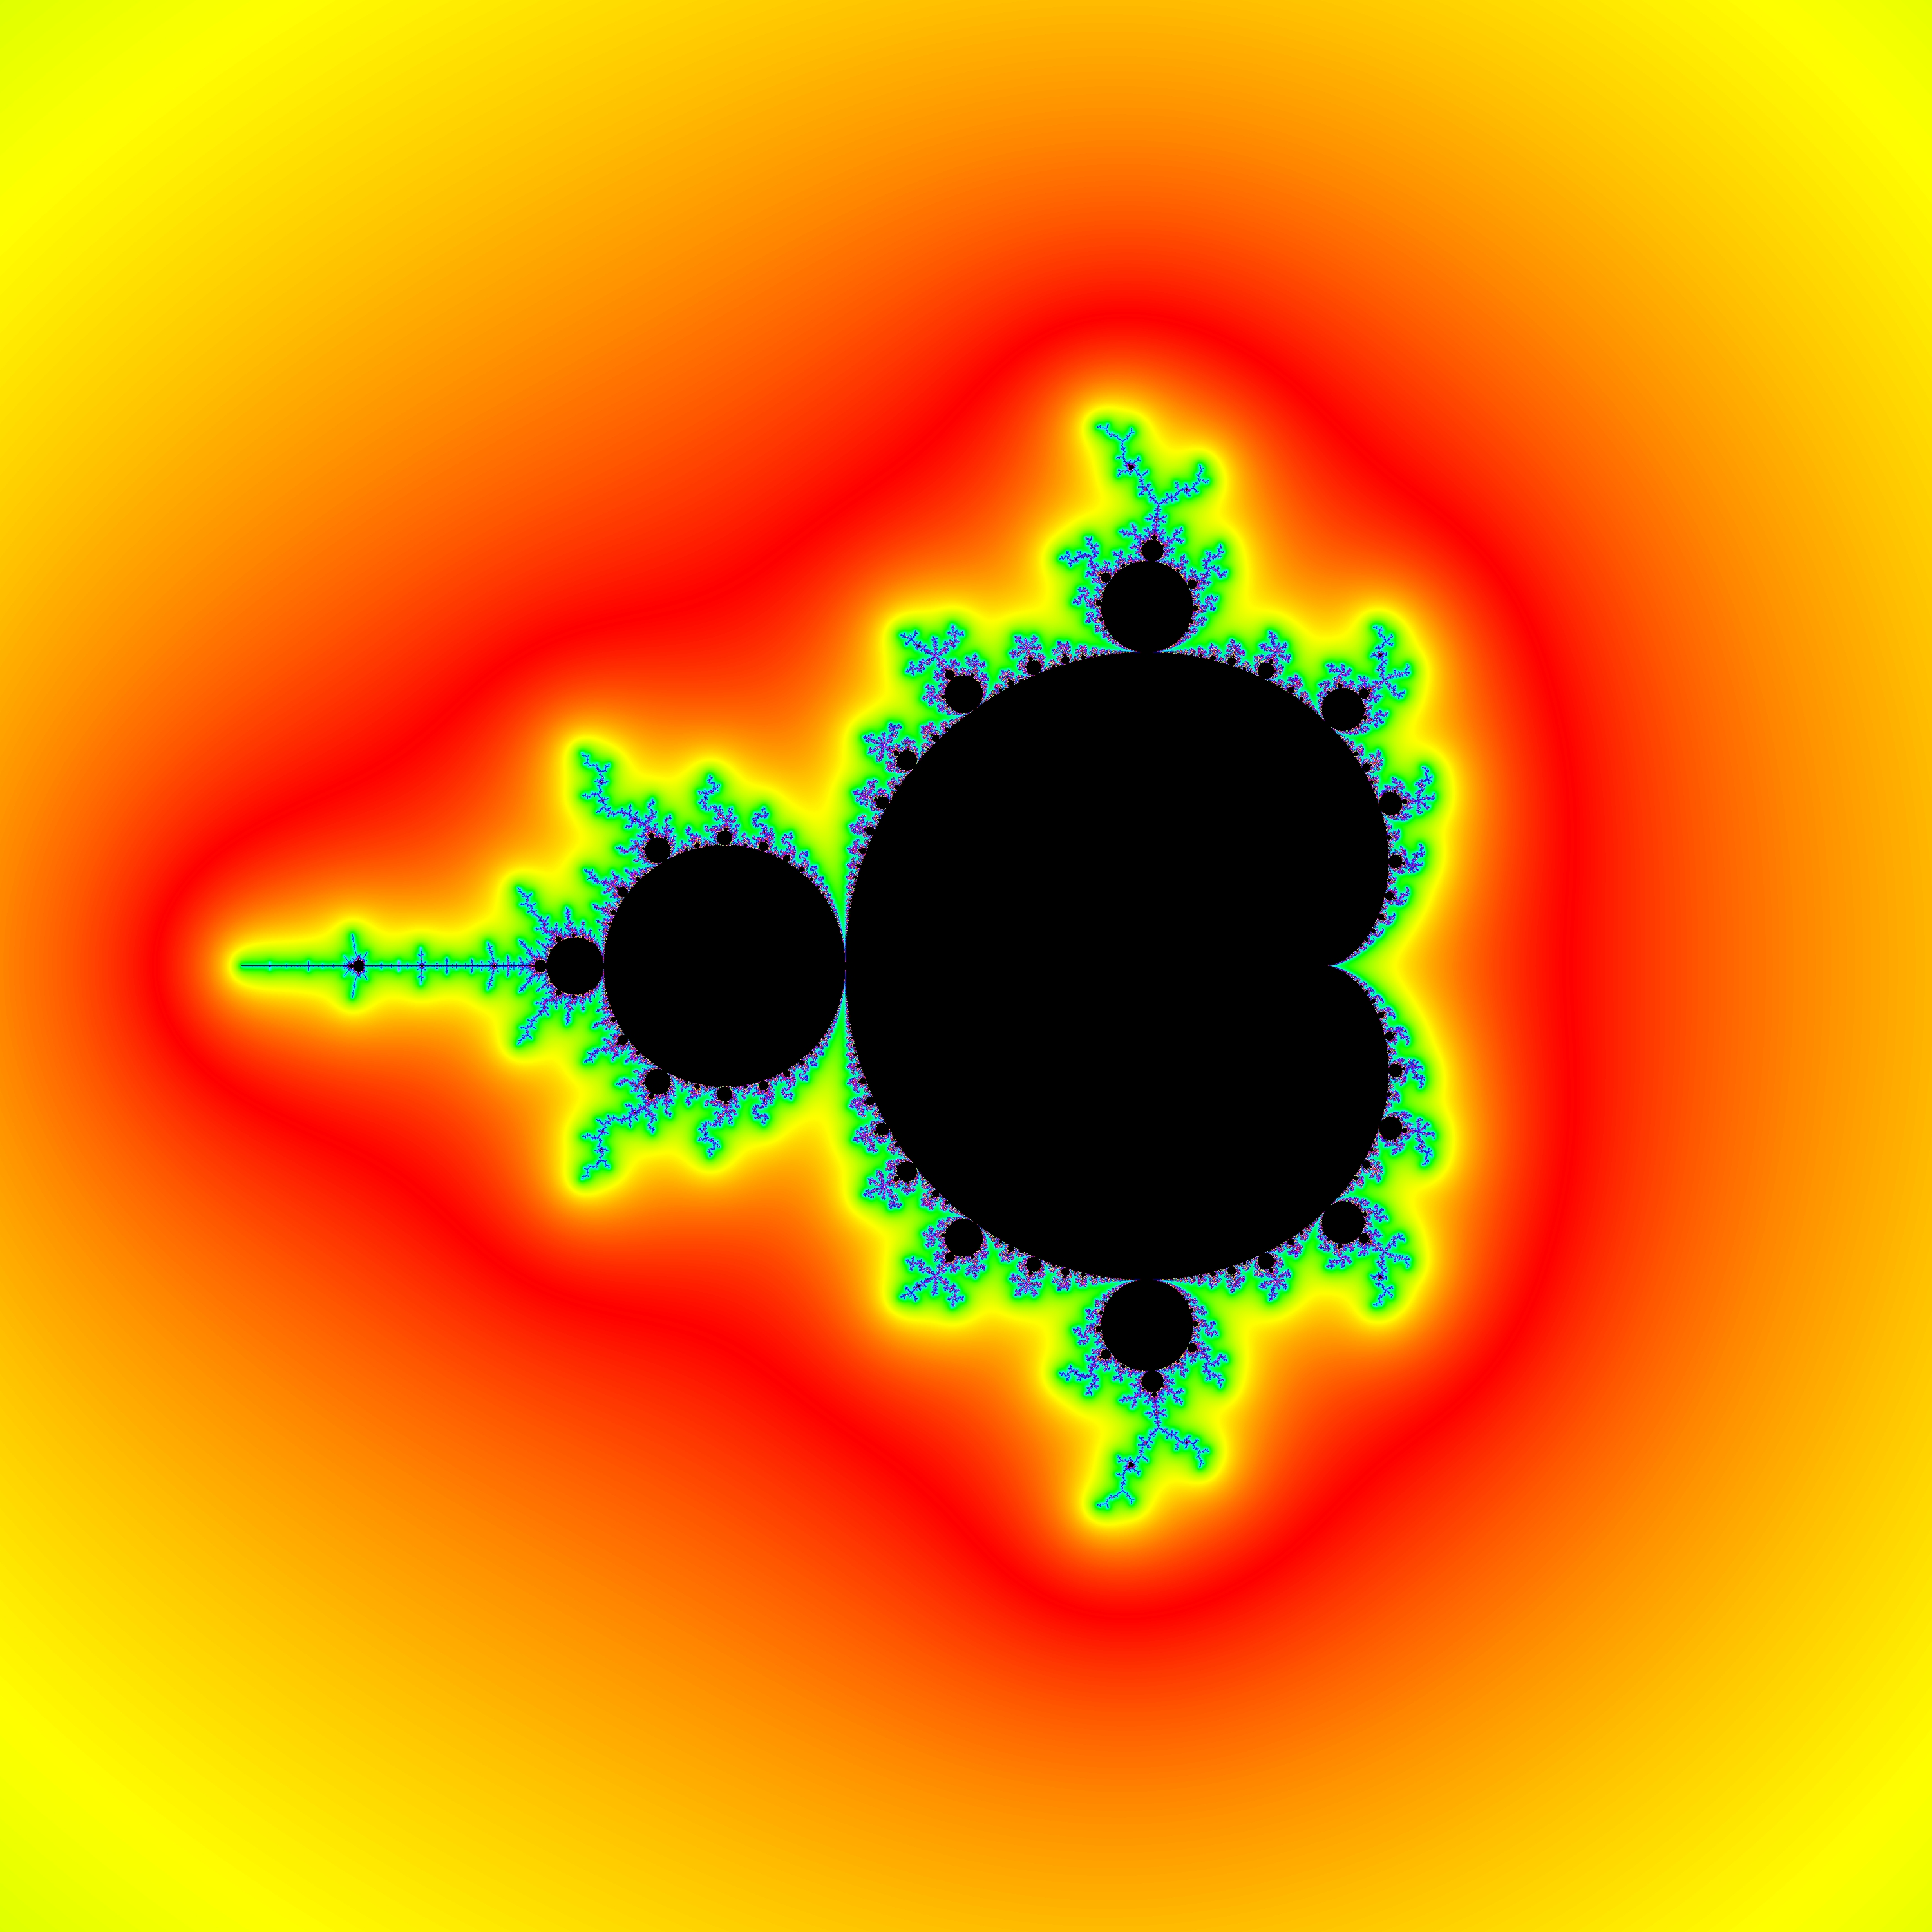
\includegraphics[width=\textwidth,trim={230 530 570 530},clip]{graphics/mandelbrot.jpg}
    \caption{The Mandelbrot set \(M\). Points \(z\in M\) are colored black. Other points are colored according to their estimated distances to \(\partial M\).}
    \label{mandelbrot_picture}
\end{figure}

The mandelbrot set is a fractal, which means that by zooming into the set similar patterns appearagain and again. A video\footnote{\url{https://vimeo.com/12185093}} shows zooming into the border of \(M\), ednoted by \(\partial M\), eventually reaching a zoom factor of \(2^{760}\). The video is not art nor kitsch; it is a visualisation of \(M\) created solely out of its definition. The colors indicate how fast the sequence corresponding to a point \(c\notin M\) diverges. (The music is not generated from the definition of \(M\).)

According to a 1991 publication\footnote{\url{https://arxiv.org/abs/math/9201282}} by M. Shishikura, the Hausdorff dimension of \(\partial M\) is two. The precise definition of Hausdorff dimension is complicated, but it can be understood intuitively.

When measuring the volume of a set in \(\RR^3\), we cover the set with small balls and add their volumes together. The smaller balls we use, the more precise estimate of the volume we get. A simple fat object has positive volume. On the other hand, its border which is a thin object has zero volume. This is because the volume of a ball is proportional to the cube of its radius \(r\) but the number of balls needed is proportional to \(r^2\), and as we use smaller and smaller balls the estimate of the volume goes to zero.

However, we can measure the area of the border by artificially changing the formula for calculating the volume of a ball from being proportional to \(r^3\) to being proportional to \(r^2\). If we want to calculate the length of a wire-like object, we use \(r^1\). If you use too low \(x\) in \(r^x\), you get \(\infty\), and isf you use too high \(x\), you get \(0\). Each set has its own correct \(x\), the Hausdorff dimension of the set.

Sets we study usually have \(x\in\NN\). The Hausdorff dimensions of a fat, thin and a wire-like object are \(3\), \(2\) and \(1\). For a simple set \(X\) the Hausdorff dimension of \(\partial X\) is less than the one of \(X\) by one. An esoteric set may have non-integer Hausdorff dimension. 

\(M\) and \(\partial M\) has the same Hausdorff dimension, two. It means that \(\partial M\) is infinitely long and extremely wrinkled. It implies that no matter how deep we zoom into \(\partial M\), we will always see complex patterns.
% note that wikipedia has decent articles of almost all mathematical concepts
% cardinality of C

We now have the countable sets \(\NN\), \(\ZZ\) and \(\QQ\) of cardinality \(\aleph_0\), uncountable sets \(\RR\) and \(\CC\) of cardinality \(2^{\aleph_0}\), proper classes \(O\) and \(\lbrace x: x\;\text{is a set}\rbrace\) and the nonexisting \(\lbrace{x:x\notin x\rbrace}\).

\section{Rigor}

Earlier in this chapter I used reasoning of variable rigorouseness. I explained Hausdorff dimension quickly and showed \(|X|<|2^X|\) somewhat carefully. It's always a tradeoff: more rigor and you get more solid results. Less rigor and you can tackle a wider set of problems. Another question from the beginning illustrates the point:
\begin{quote}
    Is it possible to comb a hairy ball?
\end{quote}
As Figure \ref{combing_hairy_ball} shows, combing a hairy ball necessarily fails at least at one point. A cowlick is necessary. No rigor is needed. Anyway, what if the ball has some other dimension? A circle
\begin{eqna}
    \setlength{\unitlength}{0.1\textwidth}
    \begin{picture}(1,1)
        \put(0.5,0.5){\circle{1}}
    \end{picture}\nonumber
\end{eqna}
can obviously be combed without cowlicks. Still no rigor needed. Anyway, in other dimensions the situation changes.

Let's start from defining the circle, or one-dimensional sphere, denoted by \(S^1\). It is a subset of \(\RR^2\) of points which all have the same distance to some specific point. Choosing this point to be the origin and the radius being one, we can, with the aid of the Pythagorean Theorem, define \(S^1\subset\RR^2\) as those points \(x_1,x_2\) for which
\begin{eqna}
    x_1^2+x_2^2=1.
\end{eqna}
A little geometry and another use of the Pythagorean Theorem shows that \(S^2\), that is the border of usual origin-centric ball of radious one, can be definied analoguously, as a subset of \(\RR^3\) of points \(x_1,x_2,x_3\) for which it holds that
\begin{eqna}
    x_1^2+x_2^2+x_3^2=1.
\end{eqna}
In general, \(S^n\subset\RR^{n+1}\) is the set of points for which
\begin{eqna}
    \sum_{i=1}^nx_n^2=1.
\end{eqna}
Here it took some rigor to define \(n\)-dimensional sphere. Which are the values of \(n\) for which the combing can be done without cowlicks? This is a highly nontrivial question and requires rigorous mathematics.

One good reason for being rigorous is generality. If we define a mathematical concept carefully, that is, we choose so-called axioms, and prove results following from those axioms equally carefully, we get a robust sets of theorems that hold \emph{always when the axioms hold}. By being once rigorous, we get solid data of any system that satisfies the axioms.

A very useful example of strictly defined mathematical concept is a group. It is a set \(G\) and a binary operation \(*:G\times G\rightarrow G\) which together satisfy the following axioms:
\begin{itemize}
    \item Associativity: for all \(a\), \(b\) and \(c\in G\) it holds that
    \begin{eqna}
        (a*b)*c=a*(b*c).
    \end{eqna}
    \item Identity element: there is an element \(e\in G\) such that for any \(a\in G\) it holds that
    \begin{eqna}
        e*a=a*e=e.
    \end{eqna}
    \item Inverse element: for any \(a\in G\) there is an element \(a^{-1}\in G\) for which it holds that
    \begin{eqna}
        a^{-1}a=a\,a^{-1}=e.
    \end{eqna}
\end{itemize}
Now we can prove carefully results that hold for any group.
\begin{teoreema}
The identity element of a group is unique.
\end{teoreema}
\begin{proof}
Let \(e\) and \(\tilde{ei}\) be identity elements. Since \(e\) is an identity, it holds that \(e*\tilde{e}=\tilde{e}\), and since \(\tilde{e}\) is an identity, it holds that \(e*\tilde{e}=e\). Therefore \(\tilde{e}=e*\tilde{e}=e\).
\end{proof}

We have already met groups. For example \(\ZZ\) with the normal addition \(+\) is a group in which \(e=0\) and \(n^{-1}=-1\). Als \(\RR\) is a group with \(+\). If we remove \(0\) from \(\RR\), it becomes a group with the normal multiplication \(\cdot\) the identity being \(1\) and inverse \(x^{-1}=\frac{1}{x}\). Also \(\lbrace\CC\setminus\lbrace{0}\rbrace,\cdot\rbrace\) is a group. The identity is \(1\) and the inverse is
\begin{eqna}
    (\theta_z,|z|)^{-1}=(-\theta_z,\tfrac{1}{|z|}).
\end{eqna}

These groups are commutative or abelian, meaning that \(a*b=b*a\). Commutativity of a group is not a theorem: there exists nonabelian groups. An important examples are rotation groups \(\mathrm{SO}(n)\) with \(n\geq3\). \(\mathrm{SO}(n)\) consists of maps \(R:\RR^n\rightarrow\RR^n\) which keep the distance of a point from the origin untouched and do not mirror.%Why is this noncommutative?

The configuration of a physical object, for example a stone, can be described by a point in \(\RR^3\), which corresponds to location, and an element in \(\mathrm{SO}(3)\). Ignoring location, we chooose some reference stone and tell how much the actual stone has rotated with respect to the reference, which fixes the \(\mathrm{SO}(3)\).

When we change the configuration of the stone---keeping it in hands while turning it in this way and that---we draw a path in \(\mathrm{SO}(3)\). Now we can ask an interesting question: is \(\mathrm{SO}(3)\) simply connected? A space being simply connected means that any loop can be continuously shrinked to a point. \(\RR^2\) is connected but \(\RR^2\setminus\lbrace0\rbrace\) is not, since a loop around the hole left by removing \(0\) cannot be shrinked.

The question may sound difficult, but the answer can be found without rigor. The method is called Dirac's belt trick. A path in \(\mathrm{SO}(3)\) can be parameterised with a belt. We get a loop if both ends of the belt are in the same configuration. We can deform loops just moving the belt while keeping the ends in the same configuration (but not necessarily in the same locations).

A unit path is a path which starts from the identity and does not rotate at all, in other words, a completely straight belt. Now, take the other end and rotate it by \(\tau\). Now you have a loop which starts from and ends at identity, but which does something in the middle. Try to deform that that into the identity. You'll find that you can't. \(\mathrm{SO}(3)\) is not simply connected.

If you take the straight belt and you twist the other end by \(2n\tau\), then you can deform it into the identity. There are two sets of loops: those that can be deformed to the identity and those that cannot. The latter ones can be deformed into each other.

This reasoning may not convince you perfectly. To be certain about the non-simply connectedness of \(\mathrm{SO}(3)\) requires rigor. Furthermore, finding simply connected \(\mathrm{SO}(n)\)'s also requires rigor.

An \(\mathrm{SO}(3)\) rotation leaves \(S^2\) intact. There's a result called Banach-Tarski paradox according to whic \(S^2\) can be split into five parts and then construct from these pieces two whole \(S^2\)'s by just rotating the pieces, provided that we can always choose. This is highly counterintuitive result: doesn't rotation preserve area? How is it possible that splitting and rotating makes two out of one?

A question from the beginning:
\begin{quote}
    Can we always choose?
\end{quote}
More precisely, if we have a collection of nonempty sets \(X_i\), is there always a function \(f\) such that \(f(i)\in X_i\), or in other words, is a Cartesina product of nonempty sets always nonempty?%is this chice function correct?

It's tempting to answer yes. It seems obvious that choosing is always possible. Yet that assumption leads to absurd results like the Banach-Tarski paradox and well-ordering of any set. This question, together with the ``set'' of all sets, ordinal numbers and Russel's paradox motivates rigorous study of sets and leads to axiomatic set theory. So-called Axiom of Choice says that yes, we can always choose. It is an axiom, not a theorem.

%For example, a bent sheet of metal satisfies the definition of a 2-dimensional Riemannian manifold, so we know that it's curvature at any point can be characterized with two real numbers, and that curvature satisfies the Bianchi identities.
%do parallel lines continue to be parallel? parallel axiom. manifolds. results: curvature tensor, bianchi identities.
% rigor is pointless if the math is intuitive or if the starting point is vague. Or if the question is boring and someone else has worked it out.

%what's wrong with math and physics teaching

%An observation: People don't write their insights down. I often get an idea, and after explaining it to others, I her, that's obvious, didn't you understand it already? I ask, why haven't you told it me! I write it down, and it's fucking perfect.


\section{Some axiomatizations}

%\section{Mechanics}

%\chapter{Our space and time}

%\chapter{To deduce and compute}

%\chapter{Linear algebra}

%examples: arrows, R^n, C^n, function spaces, spaces of linear operators, solutions of a linear differential equaition

%applications: geometry (tangent space), velocity, quantum mechanics, neural networks, cryptography, lie algebra

%\chapter{overline of mathematics}

\begin{comment}

propositional logic
set theory
coputability theory

algebra
topology

analysis
geometry
functional analysis
probability
Lie groups
algebraic topology




\end{comment}

\newpage

\subsection{Axioms of classical mechanics}

In the following \(\mathcal{M}\) is a symplectic manifold.

\begin{itemize}
    \item The state of the system is associated with a function \(\rho:\mathcal{M}\rightarrow\RR\) for which it holds that 
    \begin{eqna}
        \rho(x)\geq0\qquad\text{and}\qquad\int_\mathcal{M}\rho(x)\,\dd x=1.\nonumber
    \end{eqna}
    \item Each obervable quantity \(O\) is associated with a function \(\mathcal{O}:\mathcal{M}\rightarrow\RR\).
    \item The value of an observable quantity \(O\) in state \(\rho\) is
    \begin{eqna}
        \langle\mathcal{O}\rangle_\rho=\int_\mathcal{M}\rho(x)\mathcal{O}(x)\,\dd x.\nonumber
    \end{eqna}
\end{itemize}

\subsection{Axioms of quantum mechanics}

In the following \(\mathcal{H}\) is a Hilbert space equipped with an inner product.

\begin{itemize}
    \item The state of the system is associated with a linear, self-adjoint operator \(\rho:\mathcal{H}\rightarrow\mathcal{H}\) for which it holds that
    \begin{eqna}
        \braket{\psi|\rho|\psi}\geq0\qquad\text{and}\qquad\Tr(\rho)=1.\nonumber
    \end{eqna}
    \item Each observable quantity \(O\) is associated with a linear operator, self-adjoint operator \(\mathcal{O}:\mathcal{H}\rightarrow\mathcal{H}\).
    \item The expected value of an observable quantity \(O\) in state \(\rho\) is
    \begin{eqna}
        \langle\mathcal{O}\rangle_\rho=\Tr(\rho\mathcal{O}).\nonumber
    \end{eqna}
\end{itemize}

\subsection{Quantization}

First observe that molecular phenomena seems random. Then write classical statistical physics in a slightly different form.

\begin{itemize}
    \item Differentiable manifold \(\rightarrow\) Hilbert space equipped with an inner product
    \item Real-valued function \(\rightarrow\) linear, self-adjoint operator
    \item positive semidefinity as a function \(\rightarrow\) positive semidefinity as an operator
    \item Integral over the manifold \(\rightarrow\) trace in Hilbert space
\end{itemize}
%tytyy mainita koordinaatit -> complete setti operaattoreita, ja muut observaabelit vanhojen funktioina, ja poisson bracket -> kommutaattori, ja karteesinen tulo -> tensoritulo

%tarvitaan klassiset vastaavuudet koska limillä hbar -> 0 täytyy ilmestyy klassinen teoria

\chapter{A quest for ultimate rigor}

Russel's paradox and other absurdities drove mathematics in a foundational crisis about a cantury ago. Thanks to logicians and set theorists, the crisis has now largely been solved. I start now from the very bottomi and aim to be as rigorous as possible.

Immediately a question arises: how rigorous can we be? Many would say, ``as rigorous as we want, it's just a question of patience.'' But how can we be sure about that? Maybe wa can't be completely rigorous. Let's see how far we can get.

\section{Empirical results}

By the very definition of our task, we have nothing to begin with. No math, no logic, no god. To be honest, I don't know how to tackel the problem if it really is interpreted that strictly. \emph{Tyhjästä ei voi nyhjäistä}, as we say here in Finland.

If a child was a \emph{tabula rasa}, he or she would not learn anything. But we people are born with a language instinct in our DNA. We are no tabula rasa. The same problem is encountered in the field of machine learning and artificial intelligence: there's no general learning algorith; an algorith must always be crafted for the task it'll be used for. The ``no free lunch theorem'' of computer science gives some rigor to this notion.

Our \emph{tabula} has been written during millions of years of evolution of \emph{homo sapiens}. To get started, we must consider \emph{empirical data} of our very own thinking and try to model it. That's right: mathematics is not usually thought of as an empirical science, yet when we seek ultimate rigor, we need empirism?.

Of course, every time we do math, we use experience and data sought from the surroundings and past. We just do it instinctively, without noticing. Now we will be very explicit.

Think of a human being, say Jasmine, explaining some issue. That is our starting point. How does she do it? She talks, shows body language. It's all very vague, but we can strip off some less essential features of her presentation. It's a tradeoff: while we remove vagueness, the expressive power of the presentation goes down.

So we strip off body language and tone of voice. We change spoken language to text. The expressive power is still good---I've had deep discussions with Jasmine via just e-mail---but we can now say something definite about Jasmine's presentation: it's a finite string \(s_n\) of symbols from a finite alphabet \(A\). There's infinitely many presentations, but they are countable. (why? must be shown) There's less possible presentations than there are real numbers.

This reasoning is of course intuitive, informal, nonrigorous. It's metamathematics. We can't avoid it when seeking for rigorous foundations.

Written english is still somewhat vague. let's formalize more: a presentation can be split into sentences, each of them stating something. If Jasmine cares enough about getting her point through, she collects her conclusions into a few sentence in the end of her presentation.

Some terminology: if Jasmine reasoned correctly, her presentation is called a proof and her conclusions are a theorem. Since many sentences can be melted together, we can assume that a theorem is always a single sentence. A proof is useful to think of as a string of many sentences. Now the proof looks something like this:
%\begin{lstlisting}
%A sentence
%another sentence
%...
%one more sentence
%THEOREM
%\end{lstlisting}
\begin{quote}
A sentence. Another sentence. Third sentence! \ldots One more sentence. The theorem.
\end{quote}
Indeed, proofs in mathematical literatures are exactly of this form.

This is still a little vague. What is a sentence? How to correctly deduce more sentences?% We can single out some especially important words from a proof, for example \lstinline!if!, \lstinline!then! and \lstinline!not!.

\section{Zeroth-order logic}

Zeroth-order logic, or propositional calculus, is a formal system of reasoning which goes back to ancient Greece. In zeroth-order logic models logical relations between propositions ``Gödel was nuts'' and ``all fruits are green'' expressed by words like ``and'', ``or'' and ``not''. We could also have other things like functions and relations, but let's not consider them.

%It is astonishingly little symbols that are needed for that. We need symbols \(A,B,C\cdots\) to express propositions. Let's think there's a countably infinite number of them, although the Latin alphabet only has 26 letters. We will not need more, so it will not be a practical problem.

It is astonishingly little symbols that are needed for that. Let's take \(\NN\) to denote propositions and \(\uparrow\) to denote ``not both''. That's it! We don't need distinct symbols for ``and'', ``or'' and so on, because as we'll soon see, we can express them by using \(\uparrow\).

We could use infix notation and write formulas like
\begin{eqna}
    (1\uparrow0)\uparrow((3\uparrow8)\uparrow4),
\end{eqna} 
but we don't parenthesis if we write \(\uparrow12\) instead of \(1\uparrow2\). This Polish prefix notation is unambiguous because each \(\uparrow\) eats exactly two formulas.% We'll show this carefully soon.
\begin{maaritelma}
A formula of propositional calculus is a finite, non-empty sequence of elements from \(\NN\cup\lbrace\uparrow\rbrace\) which is either a single number or \(\uparrow\) followed by two formulas. A subformula of formula \(\psi\) is a formula which is part of \(\psi\).
\end{maaritelma}
Our example formalised to the extreme is the sequence
\begin{eqna}
    \uparrow,\uparrow,1,0,\uparrow,\uparrow,3,8,4.
\end{eqna}
\begin{lemma}[Unique readability]
Decomposition of a formula into subformulas is unique.
\end{lemma}
\begin{proof}
If formula \(\psi\) is only a number, then the decomposition is \(\psi\). Otherwise note that a proper initial segment of a formula is not a formula. jlsdjlkc
\end{proof}
If only finite alphabet is available as is in a computer environment, then we can create an effective infinite alphabet by using words instead of single letters. The extreme is of course words formed out of binary alphabet \(\lbrace0,1\rbrace\) in such away that even if concatenated, the words can be told apart. Then our formulas would be nothing but finite strings of zeroes and ones.

In any case formulas are finite sequences of symbols from a countable alphabet. We can assign a number \(n\in\NN\) to any formula by the following procedure. First map the alphabet to positive natural numbers \(\NN^+\), for example \((\uparrow,0,1,2,3,\dotsc)\mapsto(1,2,3,4,5,\dotsc)\). Our example formula would become \(1,1,3,2,1,1,5,10,6\). Then map the sequence  by taking the \(n\)th symbol to the \(n\)th prime number exponentiated to the power of \(n\)th symbol. In our example that would be
\begin{eqna}
    2^1,3^1,5^3,7^2,11^1,13^1,17^5,19^{10},23^6.
\end{eqna}
Then multiply the numbers together. In our example we get
\begin{eqna}
    6772375242492923775204255946433250.
\end{eqna}

This is called Gödel numbering. It is not unique; we can map the alphabet to \(\NN^+\) in any injective way we wish. Since prime number factorization of each \(n\in\NN\) is unique, no two strings map to the same number. In other words, Gödel numbering provides an injection from the set of formulas to \(\NN\).
\begin{lemma}
Given a countable alphabet \(A\), the set of finite sequences of symbols of \(A\) is countably infinite.
\end{lemma}
\begin{proof}
Gödel numbering provides an injection to \(\NN\), so the set is countable. There are infinite many possible lengths for a sequence, so the set is infinite.
\end{proof}
If you're about to write a book, you only have countably many possibilities.

Our formal syntax is very inconvenient to use. Let's take some informal notation to abbreviate it. We use Greek letters \(\psi,\varphi,\phi,\dotsc\) to denote formulas. We also use infix notation with enough parenthesis to make the expression unambiguous. We use the following abbreviatons:
\begin{eqna}
    {\psi\uparrow\psi}=\neg\psi,\nonumber\\
    (\psi\uparrow\xi)\uparrow(\psi\uparrow\xi)=\psi\wedge\xi,\nonumber\\
    (\psi\uparrow\psi)\uparrow(\xi\uparrow\xi)=\psi\vee\xi,\nonumber\\
    \psi\uparrow(\xi\uparrow\xi)=\psi\rightarrow\xi\nonumber
\end{eqna}
and
\begin{eqna}
    (\psi\rightarrow\xi)\wedge(\xi\rightarrow\psi)=\psi\leftrightarrow\xi.\nonumber
\end{eqna}
The symbols \(\neg,\wedge,\vee,\rightarrow\) and \(\leftrightarrow\) read ``not'', ``and'', ``or'', ``implies'' and ``if and only if''. We'll see that these interpretations make sense. The need of parentheses is diminished by the convention that \(\neg\) affetcs to only what is right next to it, that is, \(\neg\psi=(\neg\psi\), and that \(\leftrightarrow\) affects as far as it can, which is the opposite of as it is with \(\neg\).

Now we can translate an English sentence into our propositional language.
\begin{quote}
    If Python is elegant or easy, people will like it, and vice versa.
\end{quote}
Let's use \(1\) to denote the statement ``Python is elegant'', \(2\) to denote ``Python is easy'' and \(3\) to denote ``people like Python''. Then we have \(\psi=\) ``if \(1\) or \(2\), then \(3\), and vice versa``, or using symbols,
\begin{eqnb}
    \psi&=&(1\vee 2)\leftrightarrow 3\nonumber\\
    &=&((1\uparrow1)\uparrow(2\uparrow2))\leftrightarrow3\nonumber\\
    &=&[((1\uparrow1)\uparrow(2\uparrow2))\rightarrow3]\wedge[3\rightarrow((1\uparrow1)\uparrow(2\uparrow2))]\nonumber\\
    &=&[((1\uparrow1)\uparrow(2\uparrow2))\uparrow(3\uparrow3)]\;\wedge\nonumber\\
    &&[3\uparrow[((1\uparrow1)\uparrow(2\uparrow2))\uparrow((1\uparrow1)\uparrow(2\uparrow2))]]\nonumber\\
    &=&\lbrace[((1\uparrow1)\uparrow(2\uparrow2))\uparrow(3\uparrow3)]\;\uparrow\nonumber\\
    &&[3\uparrow[((1\uparrow1)\uparrow(2\uparrow2))\uparrow((1\uparrow1)\uparrow(2\uparrow2))]]\rbrace\uparrow\nonumber\\
    &&\lbrace[3\uparrow[((1\uparrow1)\uparrow(2\uparrow2))\uparrow((1\uparrow1)\uparrow(2\uparrow2))]]\uparrow\nonumber\\
    &&[((1\uparrow1)\uparrow(2\uparrow2))\uparrow(3\uparrow3)]\rbrace\nonumber
\end{eqnb}
which finally becomes (omitting commas) the sequence
\begin{eqnb}
    \psi&=&\uparrow\uparrow\uparrow\uparrow\uparrow11\uparrow22\uparrow33\uparrow3\uparrow\uparrow\uparrow11\uparrow22\uparrow\uparrow11\uparrow22\nonumber\\
    &&\uparrow\uparrow3\uparrow\uparrow\uparrow11\uparrow22\uparrow\uparrow11\uparrow22\uparrow\uparrow\uparrow11\uparrow22\uparrow33.\nonumber
\end{eqnb}
Tedious, but possible. (I don't know why I bothered to do that. It's 3.20 AM and I'm definitely not sure it's right. Anyway, it took me so long that I'm not going to take it away. Yeah, the fallacy of sunk costs.)

Now that we can translate English into zeroth-order logic formulas, we can tackle reasoning. When Jasmine presents her arguments, she first presents some assumptions and then deduces lemmas out of them. She may provide more assumptions as the presentation goes on. Then she deduces more lemmas out of assumptions and already proved lemmas finally arriving at her theorem.

Therefore a formal proof should be a sequence of formulas, each of them being an assumption or a deduction based on earlier formulas in the proof. The stereotypical deduction based on earlier results is that there's a result saying \(\psi\) holds and another result saying that \(\psi\) implies \(\varphi\). It's called Modus Ponens.

Our proof therefore stems from a set of assumptions and is a sequence of sentences \(\psi_n\) such that each \(\psi_n\) is either an assumption or there's \(\varphi\rightarrow \psi_n\) and \(\varphi\) somewhere earlier in the proof.

Some formulas, for example \(\neg\neg1\rightarrow1\) which says ``if it is not that proposition \(1\) does not hold, then it holds,'' seem to be universally valid. We choose some of such formulas as logical axioms, which we can always assume. We later discuss how to choose them.% except in fuzzy situations (fuzzy logic)

\begin{maaritelma}
A proof from assumptions \(A\) is a finite sequence of formulas \(\psi_n\) such that each \(\psi_n\) is a logical axiom or an assumption from \(A\), or there are \(l,m<n\) such that \(\psi_l=\psi_m\rightarrow \psi_n\).
\end{maaritelma}
\begin{maaritelma}
A formula \(\psi\) is said to be a theorem if there is a proof \(\psi_n\) such that \(\psi=\psi_n\) for some \(n\). If that is the case, we write \(\vdash\psi\). If \(\psi\) can be proven from assumptions \(A\), we write \(\vdash_A\psi\).
\end{maaritelma}

%Now the formal syntax is complete: we have rigorous definitions for a sentences and a proof. They are so rigorous that a computer can get them: I wrote a Python program\footnote{linkki} that checks if a string of symbols is a proof. It checks everything: that words are formed well, that sentenced are formed well, and that each line of proof is an instance of an axiom or Modus Ponens.
%\lstinputlisting[language=python,basicstyle=\footnotesize\ttfamily]{scripts/checkproof.py}

\section{Interpreting our system}
%forall = V , is an element of = K, variable = word with capital letter, constant = word with xmall letter

Now we have two languages for presenting reasoning, English and zeroth-order logic. The first can be used for explaining virtually anything, but it's also vague: a computer cannot be programmed to unambiguously decide if an English sentence is syntactically correct, nor if reasoning written in English is sensible. Propositional logic can't express much things, but at least a computer can decide the correctness of a sentence and a proof?.

If a ``\(1\) or \(0\)'' type question is well-defined doesn't necessarily mean a computer can decide if it's \(1\) or \(0\). There for example may not be skilled enough programmer available, but there's more to it.

Take any function which takes a finite string of sybols and maps it to \(\lbrace0,1\rbrace\). Let's denote the set of finite strings by \(S\) so that \(f:S\rightarrow\lbrace0,1\rbrace\). Ecah such function defines a set of \(f^{-1}(\lbrace0\rbrace)\subset X\) and each subset \(Y\subset X\) defines a function \(f_Y\) by \(f(Y)=\lbrace0\rbrace\). Therefore, there's a bijection between the set of functions and \(2^X\). \(X\) is countably infinite, so \(2^X\) is uncountable: there's uncountably many functions \(f:X\rightarrow\lbrace0,1\rbrace\).

As an aside, the set of functions from \(A\) to \(B\) is often denoted by \(B^A\). Thinking of two as the ordinal number \(2=\lbrace\emptyset,\lbrace\emptyset\rbrace\rbrace=\lbrace0,1\rbrace\), it is natural to denote the powerset of \(X\) by \(2^X\).

% must be shown very carefully and clearly that set of finite string strings from a finite alphabet is countable.
Now, we have uncountably many functions \(f:X\rightarrow 2\). If Jasmine is skilled enough programmer and she's given an \(f\), can she write a program to decide it? Her programs are finite strings of symbols from a finite alphabet, so she only can write a countable number of programs. But there were uncountably many \(f\)'s! The set of decidable problems \(f:X\rightarrow2\) is a countable subset of the uncountable set of all such problems.

The question, ``is a string of symbol a valid proof of propositional logic?'' was clearly decidable: I provided a Python program ??that decided it. Perhaps undecidable problems are esoteric and don't ask anything reasonable.

Another reasonable question is if a certain computer program halts, that is, quits running. This little Python program
\begin{lstlisting}[language=python]
print("I did halt.")
\end{lstlisting}
halts after printing ``I did halt.'' on the screen. (It claims to halt even before it has halted, but since your visual cortex delay microseconds it's only a techical proble.) Thisi one
\begin{lstlisting}[language=python]
while True:
    print("I'll never halt!")
\end{lstlisting}
won't halt, as it blusters.

EXPLANATION OF HALTING PROBLEM

Back to languages. Could we find some kind of intermediate language between propositional logic that would be easy enough for a computer to tackle, yet it would be expressive enough? What is enough is relative. I don't think we chould to require the ability express love from our language. Computers don't feel love, so obviously a language which expresses love is too difficult for a computer to understand, and for us hymans there are English, Finnish and other languages well-suited for that.% at least the syntactic correctness of a sentence should be decidable

Even statements of natural science may be too vague for a computer.  Let's say that if a language can express all informal math we deal with, for example differential calculus used in physics, we're quite happy with it. If we can also do all the reasoning about the language in the language, we're super happy. In addition to the expressive power, wether a string of symbols is a correct proof or not should be decidable. If that holds for the language, the language is said to be effective. As we found out, propositional logic is effective.

\section{Semantics}

One crucial requirement of any useful language is soundness. It means that no untrue statement is a theorem. As we noted, if we take too much axioms, we can prove anything, so to keep our languages sound, we should not take too wide set of statements as axioms.

To find out if our proposition logic is sound, we must discuss its semantics: we must interpret the formulas back into English and see which of them are true.

The final question about a language was mentioned in the first chapter.
\begin{quote}
    Can we deduce every truth?
\end{quote}
In other words, is every true statement a theorem? ``Of course,'' mathimaticians used to think, but if you think of it, it's not obvious. In a formal language proofs are decicable and therefore the demand of rigor is the highest possible---that was the whole point of developing formal logic in the first place. If every truth of our language is a theorem, then the language is said to be complete. Soundness and completeness together means that there is a one-to-one correspondence between truths and theorems.

%To sum up, we are after a system of formal logic which is
%\begin{itemize}
    %\item Powerful enough to express all math, including reasoning about the language itself.
    %\item Sound.
    %\item Effective.
    %\item Complete.
%\end{itemize}
If ther is such a language, then we can deduce at least each and every mathematical truth. If the language is not effective, then we can still deduce every mathematical truth, but we can't know wether we've done it.??

If there's no sound, effective language powerful enough, then we can't deduce every truth, not even every mathematical truth. We are forced to use at least some amount of intuition, vague common sense reasoning. Of course, that would be no disaster---we humans have a pretty decent intuition. Is there such a language is nevertheless a deep, deep question, possibly the deepest of all mathematics of all times.

Prpositional logic is not expressive enough. For example,??
\begin{eqna}
    A\rightarrow A
\end{eqna}
is strictly speaking not a theorem; rather, it is a scheme for forming theorems like \propositio!I dfs dfs! and \propositio!I N ert N ert!. There's an infinite number of such theorems and they all require their own proofs.

The problem is that propositional logic can't say ``for all such and such\ldots''. We'll fix this when we graduate to predicate logic. Anyway, propositional logic definitely gets something right, and it will be a part of predicate logic, so let's discuss semantics of propositional logic.

Semantics is how we interpret each formula and its truth. In our zeroth-order logic the task is easy: \(\uparrow\) is false if both of its inputs are true. That's what ``not both'' means. Then we can define the truth value of any sentence recursively, until we hit a sentence which is just a number. At this point we must assign a truth value to all numbers. That depends on the situation in the world: if \(1\) denotes the proposition ``it rains'', then \(1\) is true if it rains, and false if it doesn't. Therefore to each world situation we assign a function \(m:\NN\rightarrow\lbrace\text{false},\text{true}\rbrace\).

\begin{maaritelma}
Let \(m\) be a world situation and \(\psi\) a formula. If \(\psi\) is a word, then its truth value is \(m(\psi)\). If \(\psi=\alpha\uparrow\beta\) for some formlas \(\alpha\) and \(\beta\), then if both \(\alpha\) and \(\beta\) are true, \(\psi\) is false. Otherwise \(\psi\) is true.
\end{maaritelma}
Due to unique readability this is sensible recursive definition. We can now understand \(\neg,\wedge,\vee\) and \(\leftrightarrow\) as ``not'', ``and'', ``or'' and ``if and only if'': just use their definitions and the definiton above to check in which circumstances they are true. For example \(\wedge\) is true only if both its inputs are true.

An implication \(\alpha\rightarrow\beta\) is true always when \(\alpha\) is not true. It is best to be understood to mean that ``if \(\alpha\) is true, then \(\beta\) is true. If \(\alpha\) is not true, then \(\beta\) may be true or not.'' This is in harmony with Modus Ponens.

Some formulas, for example \(\neg\neg1\rightarrow1\), are true, no matter what the world situation is. Such sentences represent logically valid, universal formulas.
\begin{maaritelma}
Formula \(\psi\) is said to be valid if it is true in all world situations \(m\). If \(\psi\) is valid, we write \(\vDash X\).
\end{maaritelma}
Logical axioms are valid (if we've chosen them in a sane way). Validity of a formula is easy to check: just try all the different possibilities. If the formula has \(n\) numbers, there's \(2^n\) of them; it's easy to write a program to do tha. (Even though there are infinitely many world situations \(m\), the value of \(m\) only matters in the points that appear in the formula.) Validity in zeroth-order logic is therefore decidable and we can even write a program for deciding it easily.

This demonstrates the powerlessness of propositional logic: if we can check the truth value of a formula in each world situation by brute force, the sentence can't say anything very complicated. In real life we do reasoning because we want to be sure something holds; if all we needed to do was to check validity by using an algorithm, we would not need to reason at all.

Now we can define soundness and completeness more precicely: soundness means that every theorem is valid and completeness that every valid formula is a theorem. Soundness is needed because it's no good if correct reasoning leds to conclusions that don't hold good, and completeness would be nice, because then we would have a chance to approach knowing everything by reasoning and reasoning. Language being both sound and complete means that validity is equivalent to being a theorem, in other words, \(\vdash\psi\) always when \(\Vdash\psi\).% a or not a is always a theorem
\begin{teoreema}
Zeroth-order logic is sound.
\end{teoreema}
\begin{proof}
We need to show that given any theorem \(\psi\) and any world situation, then \(\psi\) is true. Since \(\psi\) is a theorem, it has a proof \(\psi_n\) with \(\psi=\psi_m\) for some \(m\in\NN\).

By the definition of proof, \(\psi_0\) is an axiom. Axioms are valid, so \(\psi_0\) is true. Now assume that for some \(k\in\NN\) all \(\psi_n\) with \(n\leq m\) are true. If \(\psi_{k+1}\) is an axiom, it is true. Otherwise it has been formed by Modus Ponens, that is, \(\psi_l=\psi_j\rightarrow\psi_{k+1}\) for some \(l,j\leq m\). Since \(\psi_l\) and \(\psi_j\) are both true, the definition of truth value ensures that \(\psi_{k+1}\) is true.
\end{proof}
The proof used a technique called mathematical induction: we first showed that \(\psi_0\) is true. Then we showed that if \(\psi_n\) is true with any \(n\leq k\), then also \(\psi_{k+1}\). Starting from \(\psi_0\) this condition step by step ensures that all \(\psi_n\)'s are true. This is hardly surprising; it just means that Modus Ponens conserves validity.%must show that if A = B > C, then B and C are unique.

Completeness and effectiveness are bit more interesting, yet in the case of zeroth-order logic they are also trivial. Because validity is decidable, we can take all valid formulas as our logical axioms, and then every valid formula has a trivial proof, the formula itself. Therefore,
\begin{teoreema}%or corollary
Zeroth-order logic is sound, complete and effective.
\end{teoreema}
Anyway, we can ask if there is a smaller set of logical axioms that make the logic complete and effective. Yes there is, it turns out. Take all formulas \(\psi\) such that
\begin{eqnb}
    \psi&=&\neg\neg\alpha\rightarrow\alpha,\nonumber\\
    \psi&=&(\alpha\rightarrow(\beta\rightarrow\alpha))\quad\text{or}\nonumber\\
    \psi&=&(\alpha\rightarrow(\beta\rightarrow\gamma))\rightarrow((\alpha\rightarrow\beta)\rightarrow(\alpha\rightarrow\gamma))\nonumber
\end{eqnb}
with \(\alpha\), \(\beta\) and \(\gamma\) any formulas. These are all valid and somewhat reasonable formula types; note that there are an infinite number of actual axioms. These axioms make zeroth-order logic complete. The proof\footnote{See \url{http://users.jyu.fi/~lkurittu/johdlogiikkaan.pdf}, Section 2.3. Unfortunately the proof is in Finnish. With no doubt other proofs can be fround by searching the web.} consists of developing a tedious method for constructing a proof sequence for any valid formula. It isn't illuminating nor useful since it doesn't work for more advanced languages, so I'll skip it.

Just for fun, let's prove a theorem,\(1\rightarrow1\), from these axioms. Let's use abbreviated notation to keep the proof manageable.
\begin{eqnb}
&&1\rightarrow((1\rightarrow1)\rightarrow1)\nonumber\\
&&(1\rightarrow((1\rightarrow1)\rightarrow1))\rightarrow((1\rightarrow(1\rightarrow1))\rightarrow(1\rightarrow1))\nonumber\\
&&(1\rightarrow(1\rightarrow1))\rightarrow(1\rightarrow1)\nonumber\\
&&1\rightarrow(1\rightarrow1)\nonumber\\
&&1\rightarrow1.\nonumber
\end{eqnb}
The first line is of the second axiom type. The second line is of the third axiom type and proves the third line from the first (Modus Ponens). Fourth line is of the axiom type two. Line three proves the final theorem from line four.

Let's collect the results. Propositional logic is sound, complete and effective, which is good. On the other hand, its expressible power is very modest: it can't handle the concept of ``all''. Low expressive power is reflected in the facts that a computer program can decide if a sentence is a valid or not and construct a proof for any valid sentence.

%antiteesi
%semantics of and, or and implication
\chapter{First-order logic}

To get more power, we add ``all'' to our language. Some modifications are required; instead of words we will have variables, constants and a predicate symbol. The result is called predicate logic.

\begin{maaritelma}
A variable is a finite, non-empty string from the proposition logic alphabet which is not \joukk!I!, \joukk!N!, \joukk!V! or \joukk!K! and begins with a lower case letter. A constant is the same as variable except it begins with an upper case letter.
\end{maaritelma}

To implement sentences of the type ``for all \(x\) it holds that \(A\)'', we take a new symbol \joukk!V! and write sentences of the form ``\joukk!V! \(x\) \(A\)'' with \(x\) a variable and \(A\) a sentence.

There are infinitely many propositional logic languages. They are distinguished by their predicate symbols. A predicate symbol is an object which represent some property of a fixed number of constants and variables. A predicate symbol could for example take two numbers and represent the condition that the first is smaller than the second.

For simplicity and the fact that the most important application of predicate logic, set theory, only needs one predicate symbol with two inputs, let's take our logic to include only one two-seat predicate symbol \joukk!K! motivated by the finnish word \emph{kuulua} (``to belong''). By imitating our construction it will be easy to construct of predicate logic languages with any predicate symbols.

\begin{maaritelma}
A sentence of predicate logic is a finite string of symbols for which one of the following holds:
\begin{itemize}
    \item It consists of \joukk!N!, a space and a sentence
    \item It consists of \joukk!I!, a space, a sentence, a space and a sentence
    \item It consists of \joukk!V!, a space, a variable, a space and a sentence
    \item It consists of \joukk!K!, a space, a variable or a constant, a space and a variable or a constant.
\end{itemize}
\end{maaritelma}
This clearly is a decidable definition. For instance
\begin{lstlisting}[language=joukko]
I K Bieber town V teen K teen heaven
\end{lstlisting}
is a sentence.

We also take some new informal notation. We use Greek letters \(\alpha,\beta,\gamma,\dotsc\) to denote sentences, lowercase letters \(x,y,z,\dotsc\) to denote variables and uppercase letters \(A,B,C\dotsc\) to denote constans, although exceptions to this convention may occur?.

 We write \(\forall x\,\psi\) with \(a\) a variable and \(\psi\) any sentence of sentences of the form \joukk!V <a> <psi>!. We also write
\begin{eqna}
    \neg(\forall x\neg \psi)=\exists x\,\psi.
\end{eqna}
The left-hand side reads ``it doesn't hold for all \(a\) that not \(\psi\)'' and the right-hand side reads ``there exist \(a\) such that \(\psi\)'', which are clearly the same thing. A third informal notation is \(a\Subset B\) which stands for a sentence of the form \joukk!K <a> <B>!.

We use parenthesis enough to make an expression unambiguous. which acts first so on?? We also may write \(\forall x\forall y\,\psi=\forall xy\,\psi\) and \(\exists x\exists y\,\psi=\exists xy\,\psi\).

Using this notation our example sentence would read
\begin{eqna}
    C\Subset t_1\rightarrow\forall t_2\:t_2\Subset d
\end{eqna}
with \(B=\) \joukk!Bieber!, \(t_1=\) \joukk!town!, \(t_2=\) \joukk!teen! and \(h=\) \joukk!heaven!. To be even less formal, if we read \(a\Subset b\) as ``\(a\) in \(b\)'', an English translation would sound something like ``if Bieber is in town, all teens are in heaven.'' It would not have been possible to express this in propositional logic.

% quantifing, sunbstituting yms.

\(\forall\) creates a new way to reason. If we have already reasoned that ``computer crushes data,'' in which computer is a generic computer, not pointing to any individual device, we may conclude, ``all computers crush data.'' In predicate logic this means that if we have already reasoned \(\varphi\) which has (or hasn't) a free variable \(a\), then we may deduce \(\forall a\;\varphi\).

\begin{maaritelma}
A proof in predicate logic is a finite string of symbols which consists of a concatention of sentences \(\psi_n\) separated with newline characters such that for each \(\psi_n\) one of the following conditions holds:
\begin{enumerate}
    \item \(\psi_n\) is an axiom
    \item There are \(l,m<n\) such that \(\psi_l=\psi_m\rightarrow\psi_n\)
    \item There is \(j<n\) and a variable \(a\) such that \(\psi_n=\forall a\:\psi_j\).
\end{enumerate}
\end{maaritelma}
The last option is called quantificaton. Just like in propositional logic, here we also say that a sentence \(\psi\) is a theorem if there is a proof of which last sentence \(\psi\) it is. If that is the case, we write \(\vdash\psi\). If wether a sentence is an axiom or not is decidable and we have an algorith to ecide it, then it is straightforward to write a program which checks if a string is a proof or not. If ``Is this an axiom?'' decidable, then also ``is this a proof?'' is a decidable and predicate logic is effective.

\section{Semantics}

To define semantics, we need a world situation, or model as it is usually called in predicate logic. A model is all those constants \(A\) and \(B\) for which \(A\Subset B\) hold. Since there are countably infinite number of constants, we can think of a model \(m\) as the map
\begin{eqna}
    m:\NN^2\rightarrow\lbrace\text{false},\text{true}\rbrace
\end{eqna}
in which \(\NN^2\) numbers pairs of constants. Since
\begin{eqna}
    |2^{\NN^2}|=2^{|\NN^2|}=2^{|\NN|}=2^{\aleph_0}=|\RR|,
\end{eqna}
there are uncountably many models.
% explain what recursion is

Given a model \(m\), we can define truth of any sentence recursively. If \(\psi=A\Subset B\) for some constants \(A\) and \(B\), then the truth value of \(\psi\) is \(m(A,B)\). Cases \(\neg\psi\) and \(\alpha\rightarrow\beta\) go exactly as in propositional logic.

If \(\psi=\forall x\,\phi\), then \(\psi\) is true if and only if it is true with any constant put in each free occurrences of \(x\) in \(\phi\). This is captures the essence of ``for all''. If we have \(\psi=x\Subset A\), then \(\psi\) is true if \(\forall x\;x\Subset A\). The other three cases go similarly.
\begin{maaritelma}% define substitution
Let \(m\) be a model and \(\psi\) a sentence. \(\psi\) is false, if one of the following conditions hold:
\begin{itemize}
    \item \(\psi=\neg\phi\) in which \(\phi\) is true
    \item \(\psi=\alpha\rightarrow\beta\) in which \(\alpha\) is true and \(\beta\) is false
    \item \(\psi=\forall x\;\phi\) and there is a constant \(c\) such that \(S_c^x(\phi)\) is false
    \item \(\psi=x\Subset y\) and there are constants \(A,B\) such that \(A\Subset B\) is false
    \item \(\psi=A\Subset x\) and there is a constant \(B\) such that \(A\Subset B\) is false
    \item \(\psi=x\Subset A\) and there is a constant \(B\) such that \(B\Subset A\) is false
    \item \(\psi=A\Subset B\) and \(m(A,B)=\text{false}\).
\end{itemize}
Otherwise \(\psi\) is true.
\end{maaritelma}
As in propositional logic, we say that a sentence is valid if it is true in all models. Now we cannot write a program to check the validity of an arbitrary sentence given an arbitrary model, since quantification would require checking an infinite number of possibilities.

\begin{teoreema}
If axioms are valid, then predicate logic is sound.
\end{teoreema}
\begin{proof}
Let axioms be valid. It is enough to show that given any \(\vdash\psi\) and any model \(m\), then \(\psi\) is true. Since \(\psi\) is a theorem, it has a proof \(\psi_n\) such that \(\psi=\psi_n\) for some \(n\in\NN\).

The first sentence of a proof is necessarily an axiom, so it is valid. Now assume that for some \(m\in\NN\) all sentences of in the proof before \(\psi_m\) are true. If \(\psi_m\) is an axiom, then it is valid and therefore true.

If it has been deduced using Modus Ponens, there are \(l,k<m\) such that \(\psi_l=\psi_k\rightarrow\psi_m\), and by the definition of truth value for implication it must be that \(\psi_m\) is true.

The last option is that \(\psi_m\) has been deduced by quantification. In that case \(\psi_m=\forall x\,\psi_k\) with \(k<m\) and some variable \(x\). We need to show that if \(\phi\) is true, then also \(\forall x\,\phi\) is true, that is, there is no constant \(c\) such that \(S_c^x(\phi)\) is false.

%If \(\phi=a\Subset b\) is true for some variables or constants \(a,b\), then by the definition of truth value of \(\Sub\) \(\phi\) remains true in any substitution.

%Now assume \(\phi\) is not of the form \(a\Subset b\). %
%If there's no free occurrences of \(x\) in a true \(\phi\), then \(S_c^x(\phi)=\phi\) and therefore \(\forall x\,\phi\) is true. Let's do induction on the number of free occurrences in \(\phi\). Assume that ``\(\phi\) is true \(\Rightarrow\)\footnote{``\(\Rightarrow\)'' denotes the informal ``implies''.} \(\forall x\,\phi\) is true'' holds for \(\phi\) with \(n\) free occurrences of \(x\) in \(\phi\).


%If there's no free occurrences of \(x\) in a true \(\phi\), then \(S_c^x(\phi)=\phi\) and therefore \(\forall x\,\phi\) is true. Let's do induction on the number of the free occurrences of \(x\) in \(\phi\). Assume that ``\(\phi\) is true \(\Rightarrow\)\footnote{``\(\Rightarrow\)'' denotes the informal ``implies''.} there is no constant \(c\) such that \(S_c^x(\phi)\) is false'' holds for \(\phi\) with \(n\) or fewer free occurrences of \(x\) in \(\phi\).

%If \(\phi\) has \(n+1\) free occurrences of \(x\), then \(S\)from the definition of sentence it follows that \(\phi=\forall\)

%Every free occurrence of \(x\) is on either side of a \(\Subset\). The truth value of \(\Subset\) was constructed so that if it is true, it can't change to false by substitution of a variable. Therefore 
KESKEN
\end{proof}




%reductio ad absurdum / antiteesi / proof by contradiction
%deduction theorem




 to prove that if all sentences in a proof before \(\psi\) are valid, then 






 









% Is it possible that a human can decide a problem undecidable for a computer?
% church-turing thesis
\begin{maaritelma}
Sentence \(\psi\) is an axiom of predicate logic if it holds that
\begin{eqnb}
    \psi&=&\neg\neg\alpha\rightarrow\alpha,\nonumber\\
    \psi&=&(\alpha\rightarrow(\beta\rightarrow\alpha))\quad\text{or}\nonumber\\
    \psi&=&(\alpha\rightarrow(\beta\rightarrow\gamma))\rightarrow((\alpha\rightarrow\beta)\rightarrow(\alpha\rightarrow\gamma))\nonumber
\end{eqnb}
with \(\alpha\), \(\beta\) and \(\gamma\) any sentences, or if
\begin{eqna}
    \psi=\forall a\;\phi\rightarrow S^a_C(\phi)
\end{eqna}
with \(alpha\) a sentence, \(a\) a variable and \(C\) a constant or a variable such that \(S^a_C(\phi)\) does not tie? \(x\), or if
\begin{eqna}
    \psi=\forall a(\alpha\rightarrow\beta)\rightarrow(\alpha\rightarrow\forall a\beta)
\end{eqna}
with \(\alpha\) and \(\beta\) sentences and \(a\) a variable with no free occurrences in \(\alpha\).
\end{maaritelma}


\chapter{Set theory}


%\section{Completeness theorem}

%\section{Set theory}

\part{Higher structures}

\chapter{Algebra}

\chapter{Topology}

Another elementary and important structure we can equip a set with is topology. It is a notion of nearness whitout distance which allows us to talk about convergence, which means approaching some point, and continuity of a function, which means that nearby points map to nearby points. Definition of topology is not very obvious, but the concept makes great intuitive sense. Topology captures that what is common with a torus and a coffee cup.

Given a set \(X\), set \(\mathcal{T}\subset2^X\) is called a topology on \(X\) if
\begin{itemize}
    \item \(\emptyset\in\mathcal{T}\) and \(X\in\mathcal{T}\).
    \item Any finite union of elements of \(\mathcal{T}\) is in \(\mathcal{T}\).
    \item Any intersection of elements of \(\mathcal{T}\) is in \(\mathcal{T}\).
\end{itemize}
The pair \(\lbrace X,\mathcal{T}\rbrace\) is called a topological space and the elements of \(\mathcal{T}\) open sets of \(X\).

A set \(\mathcal{B}\) of sets of \(X\) is called a basis of topology \(\mathcal{T}\) if all unions of elements of \(\mathcal{B}\) is equal to \(\mathcal{T}\). For example open intervals \(]a,b[\), \(a,b\in\RR\), form a basis and generate the usual topology and concept of nearness in \(\RR\). More generally, open balls generate the usual topology of \(\RR^n\).

A sequence \(x_n\) of points in \(X\) is said to converge to point \(x\) if for any open neighborhood \(U\) of \(x\) there is \(n_U\) such that if \(n>n_U\), then \(x_n\in U\). For example \(1,\frac{1}{2},\frac{1}{4},\dotsc\) converges to \(0\) in \(\RR\)'s usual topology.

A function \(f:X\rightarrow Y\) from a topological space to another is continuos if the preimage of an open set is open, that is, the set of all the points in \(X\) of which image is in an open set of \(Y\) is always open. Continuity means the function's value does not change abruptly.

If a function is a bijection and continuous in both directions, it is a homeomorphism. Such a function preserves openness and topology. If there's a homeomorfism between two spaces, they're said to be homeomorphic, which means they are topologically similar. A cube and a ball are homeomorphic, a cube and a square aren't.

% kaikkee shittii: tulotopologia yms

A group is said to be a topological group if the group operation is continuous in some topology.

An important topological space


Of

%algebraic structures: group, field, vector space, operator algebra, Clifford algebra, Grassman algebra
%topologies: R^n, manifold
%important combinations: group + differential manifold = Lie group, vector space + inner product + completeness = Hilbert space, differentiable manifold + metric tensor = Riemannian manifold
%tangent space: local dx's, Lie algebra

%maps: derivative: R^R->R^R, integral:R^X->R







%osdjfisjfds;lvsd sd vds  kjfd vj hvf kjd nnv kjds nvkjvnd s sd fd   df hfn nhgfn ngf gf gfnh   nf nncskj ds s 
\begin{comment}    
\chapter{Analysis}

\chapter{Geometry}
%including differential geometry (linear algebra missing, what to do?)

\begin{eqna}
    1,1,1,?,1,1,28,2,8,6,992,1,3,2,16256,2,16,16,523264,24,\dotsc\nonumber
\end{eqna}

\chapter{Probability}

\part{Elementary physics}

\chapter{Linear algebre}

\chapter{Differential geometry}

\chapter{Mechanics}


\chapter{Functional analysis}


\chapter{Lie groups}

\part{Space and time}

\part{Zooming in}

quantum

\part{Tracing back}

big bang, structure formation, nucleosynthesis, stardust, Earth, primordial soup, Homo Sapiens.


\end{comment}

\end{document}
